\documentclass{article}
\usepackage{array, booktabs, graphicx, apacite, setspace, tocbibind}
\usepackage[titletoc,toc,title]{appendix}
\usepackage[toc,section=section]{glossaries}
\usepackage[parfill]{parskip}
\usepackage{grffile}
\usepackage{tocloft}
\usepackage{titlesec}

%
\setcounter{secnumdepth}{4}


% format \paragraph{example} as a subsubsubsection
\titleformat{\paragraph}
{\normalfont\normalsize\bfseries}{\theparagraph}{1em}{}
\titlespacing*{\paragraph}
{0pt}{3.25ex plus 1ex minus .2ex}{1.5ex plus .2ex}


% automatically convert "" to ``''
\usepackage [autostyle, english = american]{csquotes}
\MakeOuterQuote{"}


% define list of equations
\newcommand{\listequationsname}{\Large{List of Equations}}
\newlistof{myequations}{equ}{\listequationsname}
\newcommand{\myequations}[1]{
   \addcontentsline{equ}{myequations}{\protect\numberline{\theequation}#1}
}
\setlength{\cftmyequationsnumwidth}{2.3em}
\setlength{\cftmyequationsindent}{1.5em}


% format appendix numbering
\renewcommand\appendix{\par
  \setcounter{section}{0}
  \setcounter{subsection}{0}
  \setcounter{figure}{0}
  \setcounter{table}{0}
  \renewcommand\thesection{Appendix \Alph{section}}
  \renewcommand\thefigure{\Alph{section}\arabic{figure}}
  \renewcommand\thetable{\Alph{section}\arabic{table}}
}


% glossary and definitions
\makenoidxglossaries

\newglossaryentry{scarce}{
	name={Scarcity},
	description={There unfortunately isn't an unlimited amount of stuff}
}


% renames "Contents" to "Table of Contents"
\renewcommand\contentsname{Table of Contents}

\begin{document}

% -------------------------------------- %
% ------------ FRONT MATTER ------------ %
% -------------------------------------- %

% title page w/o page numbers

\title{\huge ECON 102 \\ \Large \medskip Macroeconomics}
\author{Charles Clayton}
\date{\today}
\maketitle

\thispagestyle{empty}

\pagenumbering{roman}
\setcounter{page}{0}

% auto-generated front matter w/ roman page numbering

\singlespacing			\pagebreak
\tableofcontents		\pagebreak

\listoffigures		
\listoftables
\listofmyequations
\pagebreak

\printnoidxglossaries	\pagebreak

% ------------------------------------- %
% ------------ MAIN MATTER ------------ %
% ------------------------------------- %

\pagenumbering{arabic}
\onehalfspacing
\section{Introduction to Macroeconomics}

Macroeconomics studies the averages and aggregates of individual markets to look at the economy as a whole. It deals with short-run behaviour like output, employment, and inflation, and how government policy can effect these variables and steer the economy. It also deals with long-run behaviour, like economic growth, investment, and technological changes. 

According to Professor Gateman, any half-decent newspaper is going to be about 50\% macroeconomics. Furthermore, if you don't understand macroeconomics, you're uneducated and he asks that you do not vote.

\subsection{Macroeconomic Variables, $YUPie$}

\subsubsection{Output and Income, $Y$}

The measure of a nation's overall level of economic activity is the value of its total production of goods and services, ie. national income/output. Production of goods and services generates income, such that \textit{by definition} national product = national income. 

Nominal national income is defined in current dollars, but real national income is measured in constant base-period terms. Prices are held constant when computing real national income, so changes only reflect changes in quantities, not inflation. $Real = Nominal/Price$

Real national income is usually measured as \textbf{GDP}, defined as the...

\begin{enumerate}

\item \textbf{final} -- no intermediate goods
  
\item \textbf{market value} -- as determined by supply and demand

\item \textbf{of all goods and services}

\item \textbf{produced in the economy}

\item \textbf{during a defined period of time}

\end{enumerate}

Since 1965, real GDP has persistently trended upward, reflecting long-term economic growth. However, in the short turn there are fluctuations around this trend, called the business cycle. Typically the business cycle is a steep rise increase in output, followed by a period of slow growth or even falling growth. 

So nation output/national income, $Y$, is what the economy actually produces. \textbf{Potential output}, $Y^*$, is what the economy would produce if all resources (land, labour, capital) were fully employed. The difference between these, $Y - Y^*$ is the difference between the two.

When $Y > Y^*$, the economy is producing more than its potential output. Typically this means that the economy is producing at unsustainable rates. It is called an \textbf{inflationary gap}, because this scenario pushes prices up. When $Y^* > Y$, the economy is producing less than its potential. This is called a \textbf{recessionary gap}.

\begin{figure}[ht!]
\centering
\includegraphics[width=100mm]{Img/2016-07-15 23_19_30-OneNote ‎- OneNote.png}
\caption{Recessionary and Inflationary Gaps}
\end{figure}


\subsubsection{Unemployment, $U$}

To increase nation income, more must be produced, so either more workers must be employed or existing employees must become more productive. In the short run, changes in productivity are very small, so increasing production closely relates to increasing employment. 

\textbf{Unemployment} refers to the number of adult workers who are not employed but who are actively searching for a job. If you've never thought about the word employment, take a moment to consider it. It shows that that person is a resource, and as a resource they are a resource being used, or employed by the economy. Similarly, unemployment means that there are resources not being used, namely people. 

There are different kinds of unemployment. 

\begin{enumerate}

\item \textbf{Frictional unemployment} refers to constant turnover in the economy of working people. Some people quit to look for jobs elsewhere, some people are fired for showing up late, and some people just graduated and are still looking for a job. 

\item \textbf{Structural unemployment} refers to when there is a mismatch between the available jobs and the available labour force. For instance, all the teaching jobs may be in Alberta, but all the teachers are in BC. Or maybe there is need for lots of millwrights, but there aren't enough millwrights available.  

\item \textbf{Cyclical employment} refers to routine unemployment that changes with the ups and downs of the business cycle or unemployment that changes seasonally. For instance, ski instructors don't work in the summer and treeplanters don't work in the winter. Most employment data actually adjusts for these trends, called seasonal adjustments.

\end{enumerate}

From an economic perspective, the reason unemployment is so important is because human labour is the least durable commodity. If the economy having a slow year so instead of logging 10k trees, only 5k trees are logged. Then you can still log those remaining 5k trees the following year. However, if there are 100 people who are unemployed one year, the value of the labour of 100 people is lost forever. In this way, unemployment is extremely wasteful. 

\subsubsection{Productivity}

Long run growth is the result of rising employment (typically a consequence of rising population), rising stock of capital, and rising productivity. 

Generally speaking, productivity is the amount of output produced per unity of input. Typically \textbf{labour productivity} is measured, as the GDP per person employed or GDP per hour worked. The second measure is typically more accurate, because the first fluctuates with the business cycle and has gradually decreased as people choose to work less hours per year. 

Productivity is the single largest cause of rising material living standards over time, and has increased drastically in the last few decades. The higher productivity of today's workers explains why real wages (the purchasing power of a worker's earnings) are significantly higher than in the past.

\subsubsection{Inflation, $P$}

Inflation means the prices of goods are services are going up \textit{on average}. If the price of apples are going up, that's not inflation. For it to be inflation, the price of everything has to be going up. The inflation rate is the rate of change of the price level. The  price level, $P$, is often measured as the \textbf{CPI} (Consumer Price Index), which serves as an index of the average price of the goods and services that are bought by typical households. As in index, it has no units and is only useful when compared to other periods.

\begin{equation}
i = \frac{CPI_f - CPI_o}{CPI_o} \times 100\%
\end{equation}
\myequations{Inflation Rate}

We value money not for the money itself, but rather for the purchasing power of the money -- its real value. Inflation reduces the real value of money. 

\subsubsection{Interest Rates, $i$}

Interest is the cost of borrowing money. The interest rate is the price paid per dollar borrowed per period of time. It is related to the opportunity cost that the bank is giving up by not investing the money elsewhere and the risk. A bank will lend money to an industrial customer at a lower rate than individuals because there is lower risk of the business defaulting on the loan. 

"The" interest rate, that economists talk about, is the mean of all interest rates in the economy. The prime interest rate is the rate that banks charge their best customers. The bank rate, is the interest rate that the central bank charges commercial banks. 

The nominal interest rate is the price paid per dollar borrowed per period of time. However, this doesn't take into account the inflation rate. Let's say you borrow \$100 at a nominal interest rate of 10\%. If the inflation rate for that year is high, say 15\%, when you pay back the \$110, even with the extra \$10, the amount repaid is worth less than when it was borrowed. 

The real interest rate takes inflation into account:

\begin{equation}
i_{real} = i_{nominal} - inflation
\end{equation}
\myequations{Real Interest Rate}

In the recession of 2008, banks became reluctant to lend money worried that businesses would not be able to pay back the loan. So market interest rates spiked upwards, which meant firms who needed credit had to reduce production and employment. 

\subsubsection{Exchange Rates, $e$}

The exchange rate is the amount of domestic currency required to purchase one unit of foreign currency. It can be thought of as the price of foreign currency, for instance 1 Euro = 1.43 CAD and 1 peso = 0.07 CAD. 

In the context of exchange rates, depreciation means that it takes more domestic currency to purchase foreign currency -- rise in the exchange rate. Conversely, appreciation means that it takes less domestic currency to purchase foreign currency -- decrease in the exchange rate.


\section{Measurement of National Income}

\subsection{Value Added}

To determine the total value of a nation's output, you can't just add up the market values the output of every firm. This is because some outputs for firms are inputs for other firms, these are called intermediate goods, and we can't double count them. 

For instance, say a farmer sells a pound of flour to a baker for \$10, and then the baker produces five loaves of bread and sells them all for a total of \$15. It's tempting to say \$10 + \$15 = \$25 of output was generated. However, we're counting the worth of the flour twice here, once by itself and once inside the bread.  

Rather, we sum the \textbf{value added} by each firm to determine the value of the total output. 

\begin{equation}
valueAdded = revenue - factorPayments
\end{equation}
\myequations{Value Added}

\subsection{Measurement of National Income}

National income, GDP, can be calculated three ways.

\begin{enumerate}

\item Add up the value added of all goods and services produced in the economy by each firm. This would give us the value of all domestic output. 

\item Add up the total value of expenditure. 

\item Add up the total value of  income. 

\end{enumerate}

By definition, all three of these will yield the same result because of the circularity of the economy. 

\begin{equation}
GDP = valueOfOutput = valueOfExpenditure = valueOfIncome 
\end{equation}
\myequations{GDP Equivalences}

\begin{figure}[ht!]
\centering
\includegraphics[width=120mm]{Img/2016-07-15 23_19_48-OneNote ‎- OneNote.png}
\caption{Circular Flow Diagram}
\end{figure}


The first method is not used because it requires know the product of every single firm and knowing the cost of all of their factors to determine the value added to avoid double counting and its just too much data. So we will discuss how GDP is calculated using methods 2 and 3 in more detail. 

\subsubsection{GDP from the Expenditure Side}

Total expenditure has been broken up into the sum of four broad categories. It's important to realize these categories and equalities have been created definitionally to include everything, they're not innate or anything. 

\paragraph{Consumption, $C$}

Expenditure by final users on all goods and services bought in the year.

\paragraph{Investment, $I$} 

Expenditure on goods not for present consumption like Inventories, or on goods to produce other goods like new Plants, new Equipment, and new Residential housing (PEIR).

\paragraph{Government Purchases, $G$} 

This includes all government purchases of goods and services, like roads and salaries of government workers. However, transfer payments, like welfare or pension plan payments, although included in expenditure are not included in government purchases.

Also, note that presumably the value of a road built by the government is more valuable than the cost to build it, otherwise they would not have built it. However, since its free we don't know the actual value, so with government purchases we value them at cost.

\paragraph{Net Exports, $NX$} 

\textbf{Imports $M$} are domestic expenditure on foreign goods and services. These add to total expenditure. \textbf{Exports $X$} are foreign expenditure on domestic goods and services. These subtract from total expenditure. So net exports, $NX = X - M$. 

Summing all these different expenditures gives us the national income.

\begin{equation}
Y = C + I + G + NX
\end{equation}
\myequations{GDP from the Expenditure Side}

\subsubsection{GDP from the Income Side}

By definition, total income is equivalent to total expenditure. It has similarly been broken into the broad categories Factor Payments and Non-Factor payments. 

\paragraph{Factor Payments}

The factors of production are Labour, Land, Captial, and Technology/Entrepreneurship. Each of these generate income via, respectively.

\begin{enumerate}

\item \textbf{Wages} -- The pre-tax income, including pensions, benefits, etc. that households receive for labour.


\item \textbf{Rent} -- Income households receive for renting land.

\item \textbf{Interest} -- Income households receive for lending money to firms (excludes income from government bonds).

\item \textbf{Profits} -- Income households receive for entrepreneurship. These include distributed profits (dividends) and undistributed profits (retained earnings). 
 
\end{enumerate}

\paragraph{Non-Factor Payments}

When a consumer spends \$10, less than \$10 is generated as income for the factors of production. This is because of two non-factor payments.

\begin{enumerate}

\item \textbf{Indirect business taxes} -- These are consumption taxes collected by business such as GST and PST, not income taxes. 

\item \textbf{Subsidies} -- These are similar to consumption taxes but they are the \textit{opposite}, they are negative taxes, so they must be subtracted.

\item \textbf{Depreciation} -- This is the loss in value of capital via wear and tear. We include this in GDP, but exclude it in Gross \textit{National} Product.

\end{enumerate}

 \begin{equation} \label{eq1}
\begin{split}
GDP & = FatorPayments + NonFactorPayments \\
    & = WRIP + (IBT - Sub) + Dep \\
\end{split}
\end{equation}
\myequations{GDP from the Income Side}

\subsubsection{Other Measures of an Economy}

\paragraph{Gross National Product, GNP}

GDP measures the value of all production in a region, say Canada. It is a  indicator of domestic economic activity in a country. GNP on the otherhand, is a measure of income received by Canadians.  It is an indicator of the economic-well being of a nation's citizens. 

For instance, a Toyota factory owned by Japanese business located in Canada would increase Canadian GDP because the production is in Canada, but it would not increase the GDP of Japan. However, the factory would increase the GNP of Japan, but not Canada. 

\paragraph{Disposable Personal Income, DPI}

Although GNP and GDP are indicators of overall economic activity and national income, disposable personal income is an indicator of individual households' ability to spend or save. In recent years, it is approximately 60\% of GDP.

\begin{equation}
DPI = Y_d = GDP + Transfer\ Payments - Taxes - Depreciation
\end{equation}
\myequations{Disposable Personal Income}

\paragraph{GDP Deflator}

Nominal GDP is valued at current prices. Any change in quantities or changes in prices will influence nominal GDP. Real GDP is valued at some base-period prices, as such only changes in quantities are reflected in real GDP. 

So by comparing changes in real and nominal GDP, we can isolate the effect of changing prices. This gives us an index number that shows the average change in price of all items in an economy. 

\begin{equation}
GDP\ Deflator = \frac{Nominal\ GDP}{Real\ GDP}\times 100
\end{equation}
\myequations{GDP Deflator}

GDP deflator is similar to CPI, but CPI reflects the prices of specifically consumer goods whereas GDP deflator reflects the prices of all goods produced in Canada. 

\paragraph{Omissions from GDP}

GDP does not measure illegal activity unless it is laundered, so although cocaine production in Columbia may generate significant income to Columbia, it is not reflected in GDP. Similarly, cash or under the table transactions are not included in GDP, even if legal. 

Additionally, \textbf{home production} -- DIY contributions to the economy are not included in GDP. If a person pays a plumber to fix a leaky sink, that service is included in GDP, however if the homeowner fixes it themselves, it is not included in GDP. Volunteer work similarly is not included in GDP. 

***

These omissions are not that important, because ultimately the importance of GDP is not the absolute number, rather it is the ability to monitor the change in production throughout the years. 

\section{Simple Short-Run Model (C and I)}

In this short-run model, we assume that national income (GDP or $Y$) is constant. We also assume that the price level is constant, so there is zero inflation. We will also, for simplicity, ignore the effects of $G$ (taxes) and $NX$ (trade).

\subsection{Aggregate Expenditure}

We will distinguish between desired and actual expenditure with the subscript $a$ for actual. Desired expenditure refers to how much people would like to spend given the resources they actually have, not how much they would spend if they won the lottery. Actual expenditure is predictably what they actually spend. 

\textbf{Aggregate expenditure}, $AE$, is the sum of all actual spending in an economy, as in equation (5), and $AE$ is a function of national income, $Y$. 

\begin{equation}
AE = C + I + G + NX = f(Y)
\end{equation}
\myequations{Aggregate Expenditure}

\subsubsection{Autonomous vs. Induced Expenditure}

Autonomous variables are elements of expenditure that do not depend on $Y$. For instance, the level of exports do not depend on national income, rather they depend on the national income of the country importing the exports. So exports are autonomous, or \textbf{exogenous variables}.

On the otherhand, some elements of expenditure do depend on national income such as imports. These elements are induced, or \textbf{endogenous variables}.

\subsection{The Consumption Function, $C$}

Since we have excluded government from our simple model, there is no taxation and so disposable income, $Y_d$, is equal to national income, $Y$. The only possible uses of disposable income are consumption and \textbf{savings} -- disposable income not yet spent on consumption. 

Desired consumption is influenced by wealth (the value of all assets minus debts), interest, and expectations about the future. However, in this model we hold the Wealth, Expectations, and Interest Rates (WEI) variables constant. So desired consumption in a function of disposable income. Additionally, because disposable income is equal to national income in this model, desired consumption is a function of disposable income.

\begin{equation}
C_d = f(Y_d)
\end{equation}
\myequations{Consumption Function}

\begin{figure}[ht!]
\centering
\includegraphics[width=70mm]{Img/2016-07-15 23_20_23-OneNote ‎- OneNote.png}
\caption{Consumption Function}
\end{figure}

\subsubsection{Slope}

The consumption function has a slope of $\Delta C / \Delta Y_d = MPC$, \textbf{marginal propensity to consume} -- the additional inclination to spend with the increase of income. MPC is constant, and positive.

The average propensity to consume is the ray from the origin to the point on the consumption function, $C/Y_d = APC$. This gradually decreases as we move along the consumption function.

\subsubsection{Shifts}

Note, changes in $Y_d$ (induced variable) cause movement along the the curve, shifts are caused by the autonomous variables.

\begin{equation}
\begin{split}
W\uparrow & \ C\uparrow \\
i\downarrow & \ C\uparrow \ \textsl{especially durable goods} \\
Optimism\uparrow & \ C\uparrow \\
\end{split}
\end{equation}
\myequations{Shifts in Consumption}

\subsubsection{The Savings Function}

The savings function has a slope of $\Delta S / \Delta Y_d = MPS$, \textbf{marginal propensity to spend}. MPS is constant and positive. 

Note that because all income must be used either to save or consume

\begin{equation}
\begin{split}
MPC + MPS = 1 \\
APC + APS = 1
\end{split}
\end{equation}
\myequations{MPS, MPC, APC, APS}

In other words, the vertical distance between the consumption function and the 45 degree line is the amount of desired savings.

\subsection{Investment Function, $I$}

Investment is the most volatile component of GDP. The variables that affect investment expenditures are Interest rates, Changes in sales, and Business Confidence (ICBC) variables. 

\subsubsection{Slope}

Note that it does not depend on $Y_d$, thus I is autonomous with respect to $Y$. As such, it is a horizontal line with a slope of zero.

\subsubsection{Shifts}

Although horizontal, it is not fixed. It can be shifted up or down by the ICBC variables. Note, recall from section 2.2.1 we say investment, we do not mean in banks, we mean in  Plants, Inventories, Equipment, and Residences. Thus when the interest rate is higher, the opportunity cost of borrowing is high, and so people do not invest in the PIER variables.

\begin{equation}
\begin{split}
i\downarrow & \ I\uparrow \\
Increase\ in\ sales\uparrow & \ I\uparrow \\
Business\ Confidence\uparrow & \ I\uparrow \\
\end{split}
\end{equation}
\myequations{Shifts in Investment}

\subsection{Aggregate Expenditure Function, $AE$}

The AE function is constructed by summing the C and I functions. It relates the level of desired aggregate expenditure to the level of actual, \textit{not nominal}, national income.

$$AE = C + I$$

\begin{figure}[ht!]
\centering
\includegraphics[width=70mm]{Img/2016-07-15 23_20_36-OneNote ‎- OneNote.png}
\caption{Aggregate Expenditure Function}
\end{figure}

\subsubsection{Slope}

The slope of the AE function is the \textbf{marginal propensity to spend} -- the additional amount of total expenditure induced when national income rises. This is different from the MPC -- the additional amount of consumption induced when households disposable income rises. 

\begin{equation}
MPSpend = z = \frac{\Delta E}{\Delta Y}
\end{equation}
\myequations{Marginal Propensity to Spend}

\subsection{Equilibrium National Income, $Y_e$}

This stable equilibrium occurs when the actual national income is equal to the level of desired aggregate spending, $AE = Y_a$. Alternatively, we could define this as when the level of withdrawals (savings) from the economy equals the number of injections (investments), $W = J$. 

If firms are able to produce any amount of output demanded of them without changing the price of their products, the output is said to be \textbf{demand determined}. 

If firms are producing at an output of \$100 billion, then the actual national income is \$100 billion, but suppose the desired aggregate expenditure is \$150 billion. In this case, $Y_a < AE$ and so firms would have falling inventories, and would have to increase output to avoid shortages, so national income would rise.


If firms are producing at an output of \$100 billion, but the desired aggregate expenditure is now \$50 billion. In this case, $Y_a > AE$ and so firms would have rising inventories, and would have to decrease output to avoid surpluses, so national income would fall.

At $AE = Y_a$, the national income is said to be at $Y_e$. Note that $Y_e$ is not important for any reason other than the fact that it is the point at which national income doesn't want to change.

\subsubsection{Shifts in Equilibrium National Income}

So $Y_e$ doesn't want to change, but it can and much effort is put into ensuring it does.

If the AE function shifts up, it intersects the 45 degree line further along the x-axis, increasing $Y_e$. The AE function shifts upwards whenever the C or the I functions increase. 

\begin{figure}[ht!]
\centering
\includegraphics[width=110mm]{Img/2016-07-15 23_20_56-OneNote ‎- OneNote.png}
\caption{Shifts in AE Function}
\end{figure}


The equilibrium point can also change if the AE function rotates. Recall the slope of the AE function is the MPS, and so as MPS increases, AE becomes steeper and $Y_e$ increases.

\subsection{Simple Multiplier}

A change in AE increases $Y_e$ by more than the initial change in AE. Your national product increases by more than your aggregate expenditure, so you get what you put in plus a little bit extra. This multiple is called the simple multiple, $k$.

\begin{figure}[ht!]
\centering
\includegraphics[width=100mm]{Img/2016-07-15 23_21_11-OneNote ‎- OneNote.png}
\caption{Simple Multiplier}
\end{figure}


Let's say a Canadian company spends \$10 million to construct a factory. This would increase national income by \$10 million, but on top of that, the increase in national income would cause an increase in desired consumption because suddenly the carpenters and factories workers have a little bit extra money. So they each buy a TV for their bedroom, so then the TV producers increase production to meet this demand, and so on. 

For the increased expenditure, there is larger amount of national income generated. This is dependent on the marginal propensity to spend, $z$, where the higher the $z$, the more significant the multiplier.

\begin{equation}
k = \frac{\Delta Y}{\Delta A} = \frac{1}{1 - z}
\end{equation}
\myequations{Simple Multiplier}

\section{Adding Government and Trade to Our Model (G and NX)}

The government can use taxing and its spending powers to affect the level of national income, called \textbf{fiscal policy}. Additionally, external affairs relating to foreign trade affect the economy. 

Here we keep our assumption that prices are fixed, so inflation has no effect. 

\subsection{Government}

\subsubsection{Government Purchases, $G$}

Government purchases, like before, include all government spending excluding transfer payments, plus government investments. All government purchases are included in GDP as goods or services, so $G$ is a direct component of $AE$. 

We will make the assumption that $G$ is not dependent on the level of national income, rather, it is a function of elections and ideology, so we will treat it as autonomous. 

\subsubsection{Taxation Revenue, $T$}

$T$ do not add directly into $AE$ because they are not an expenditure on goods and services, however taxes indirectly influence $AE$ because they decrease disposable income, $Y_d$, whereas transfer payments increase $Y_d$. Net taxes are the difference between tax revenue and transfer payments. 
\begin{equation}
\begin{split}
Y_d & = Y - (Net\ taxes) \\
& = Y - (T - TP)
\end{split}
\end{equation}
\myequations{Disposable Income and Taxes}

Typically taxes are a function of national income so we will treat net taxes, $T$, as an induced variable. The \textbf{net tax rate} $t$, is the increase in tax revenue given increase in national income, $T = tY$. It is not, however, the income-tax rate because it reflects all taxes from all levels of government. 

\subsubsection{Budget Function}

The government budget is the different between total government revenue and total government expenditure. This represents the level of money going into \textit{the government}. Note that in the circular flow diagram this is the opposite, taxes are negative and government expenditures are positive.

\begin{equation}
Budget = T - G 
\end{equation}
\myequations{Government Budget}

\begin{figure}[ht!]
\centering
\includegraphics[width=60mm]{Img/2016-07-15 23_21_29-OneNote ‎- OneNote.png}
\caption{Government Expenditure and Taxes}
\end{figure}


When revenues exceed expenditures, $T > G$, the government is running at a budget surplus. In which case the government buys back standing government debt. 

When expenditures exceed revenues, $G > T$, the government is running at a budget deficit. In this case, the government is required to borrow funds -- through bonds or Treasury bills. Although deficits have negative connotations, when looking at the circular flow diagram it can be seen that government is actually injecting more money into the flow, increasing GDP. Deficits are often run in this case to stimulate the economy. 

\subsubsection{Net Export Function}

As we said before, exports are not dependent on $Y$ although imports are dependent on $Y$. This is because consumption rises with national income and so imports rise to satisfy that consumption at the \textbf{marginal propensity to import}, $m$. 

$$M = mY$$

When $X > M$, money is going into the circular flow and so GDP rises. When $M > X$, money is leaving the circular flow. 

\begin{figure}[ht!]
\centering
\includegraphics[width=80mm]{Img/2016-07-15 23_21_39-OneNote ‎- OneNote.png}
\caption{Shifts in Net Exports}
\end{figure}

\paragraph{Shifts}

An increase in foreign income leads to wealthier foreign nations, which will result in an increase in the quantity of goods demanded by that nation, and thus an increase in Canadian exports, and finally an increase in $AE$. 

A decrease in Canadian prices relative to foreign nations, means that Canadian goods appear cheaper from outside, and so exports will increase and imports will rotate downward -- NX moves up and becomes flatter.

An increase in relative Canadian prices will lead to $X$ shifting down and $M$ rotating upward -- NX moves up and becomes steeper.  

\begin{equation}
\begin{split}
Foreign\ income \uparrow & \ NX \uparrow \ \textsl{in parallel}  \\
Relative\ Canadion\ prices \downarrow & \ NX \uparrow \ \textsl{also gets flatter} \\
\end{split}
\end{equation}
\myequations{Shifts in Net Exports}

\subsection{Equilibrium National Income}

Finally, the conditions for equilibrium is our original equation for aggregate expenditure. 

$$ Y = C + I + G + NX $$

Or restated in terms of injections and withdrawals

\begin{equation}
S + T + M = I + G + X 
\end{equation}
\myequations{Equilibrium Injections and Withdrawals (STM IGX)}

The slope of the $AE$ function is the marginal propensity to spend, $z$. With the inclusion of government and foreign trade, the formula changes. Recall $m$ is the marginal propensity to import and $t$ is the tax rate. 

\begin{figure}[ht!]
\centering
\includegraphics[width=110mm]{Img/2016-07-15 23_21_59-OneNote ‎- OneNote.png}
\caption{Injections and Withdrawals}
\end{figure}


\begin{equation}
z = MPC(1 - t) - m
\end{equation}
\myequations{Marginal Propensity to Spend}

\subsubsection{Multiplier}

Now having included government and trade, the marginal propensity to spend is not simply equal to the marginal propensity to consume. 

This is because 1) due to taxation, disposable income does not increase in equal measures as income, so consumption does not increase as much; and 2) because an increase in income results in an increase in imports, not all expenditure goes into the circular flow diagram, some goes into other countries.

In other words, increasing Y also increases T and M, which are withdrawals. This reduces the value of the multiplier, so we are now getting less out for the same amount in.

\begin{equation}
\begin{split}
k & = \frac{1}{1 - z}  												\\
  & = \frac{1}{1 - MPC} 		 \ \ \ \textsl{without G and NX}  	\\
  & = \frac{1}{1 - [MPC(1-t)-m]} \ \ \ \textsl{with G and NX}  		\\
\end{split}
\end{equation}
\myequations{Simple and Less Simple Multiplier}

Note that the steeper the $AE$ curve, the lower the multiplier is.

\section{Output and Prices in the Short Run}

Before we assumed price levels were constant, now we take changes in price level into account -- price level in an endogenous variable because its changes are explained in the model.

Changing price levels affect the desired aggregate expenditure -- the demand side of the economy, and the price of factor inputs and the level of output of suppliers -- the supply side of the economy.

\subsection{Demand Side of Economy}

\subsubsection{Shifts in AE}

Consider an increase in price level.

\paragraph{Changes in Consumption}

An increase in price levels reduces the real wealth of a household, and thus reduces desired expenditure. 

Many assets are held in money, which is then reduced in real value when price levels increase. However many assets are also fixed nominal value bonds, and when the price level rises the value of these bonds decreases. However, while the bondholders lose and the bond issuers win, the net change in aggregate wealth is nothing.

So the AE curve shift down. 

\paragraph{Changes in Net Exports}

When domestic prices rise, domestic goods become more relatively expensive, so the consumers of a country typically purchase more foreign goods, no $M\uparrow$. On top of that, foreign purchases see the goods are more expensive relative to other countries, so $X\downarrow$. Thus $NX\downarrow\downarrow$. 

So the AE curve shifts down.

\subsection{Changes in Equilibrium GDP, $Y_e$}

Downward shifts in AE due to rising price levels reduces the equilibrium level of GDP.

\begin{figure}[ht!]
\centering
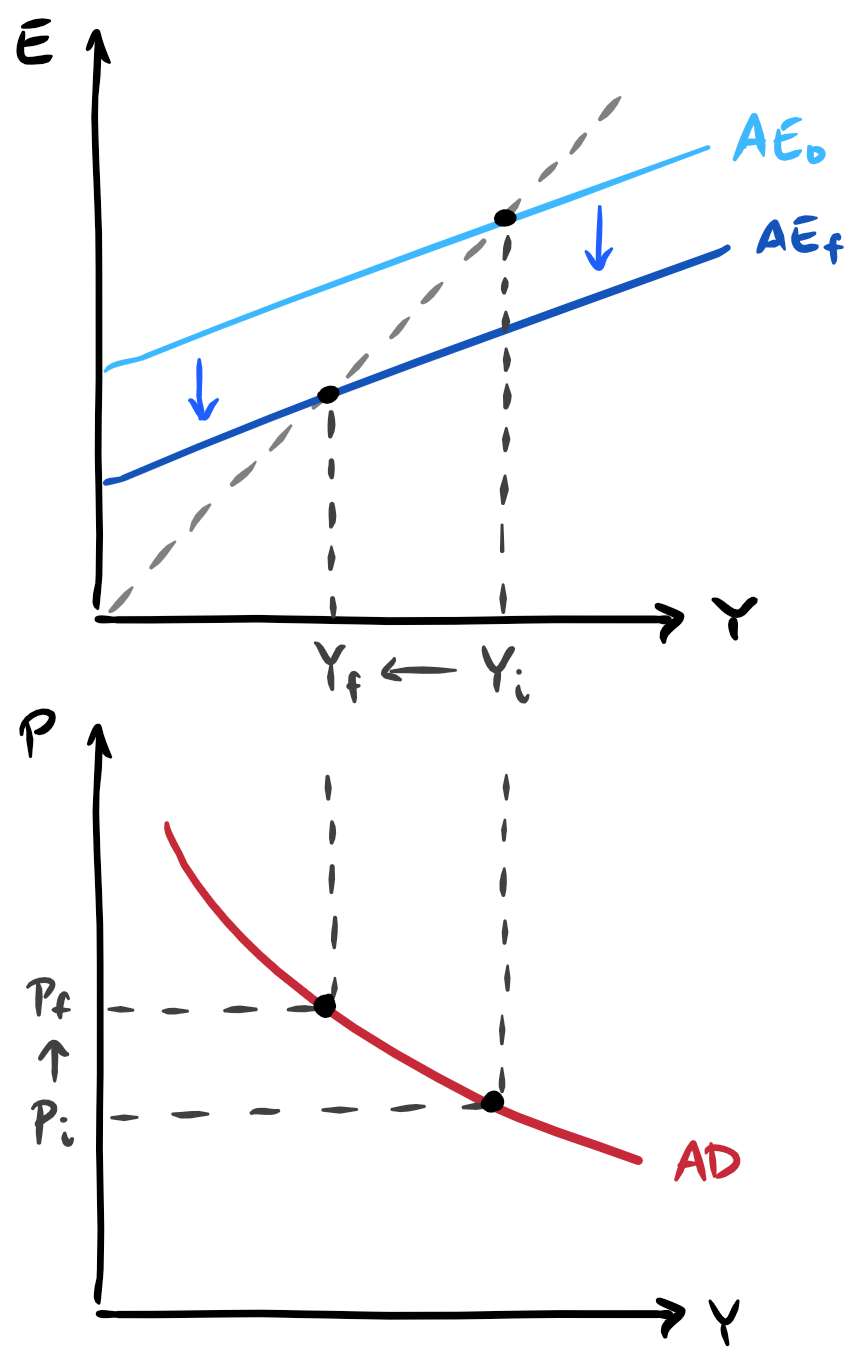
\includegraphics[width=60mm]{Img/23-2.png}
\caption{Shift in AE due to Price Change}
\end{figure}


\subsection{Aggregate Demand Curve, $AD$}

The AD curve is the relationship between the price level and the real equilibrium GDP. Price level is on the vertical axis and real GDP on the x axis. 

It shows the combinations of real GDP and the price level at which desired aggregate expenditure is equal to actual national income. 

As $P$ increase, $Y_e$ decreases. Note, it looks like the microeconomics demand curve but it's for different reasons. 


\subsubsection{Slope of AD}

It is negatively slope for two reasons.

\begin{enumerate}

\item A fall in price level leads to a rise in private sector wealth, increasing consumption, increasing equilibrium GDP.

\item A fall in price level leads to a rise in exports and a decrease in imports, increasing equilibrium GDP. 

\end{enumerate}

\subsubsection{Shifts in AD}

Any event that changes equilibrium GDP, or shifts the AE curve, other than a change in price will cause the AD curve to shift. This is called an aggregate demand shock. 

\begin{figure}[ht!]
\centering
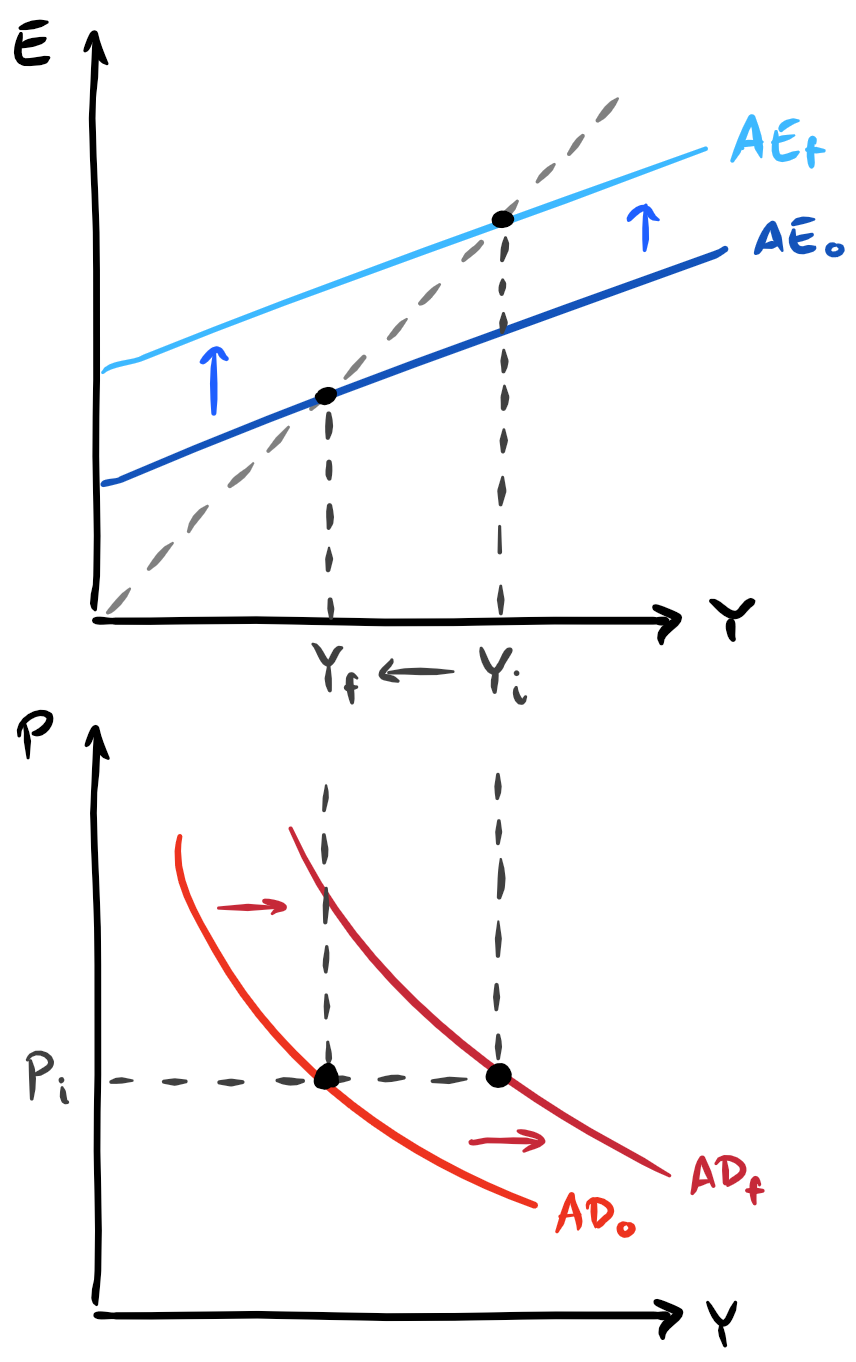
\includegraphics[width=60mm]{Img/23-3.png}
\caption{Shift in AE due to Shift in AD}
\end{figure}

Such as government purchases or taxation, or change in consumption, or investment behaviour. 

Keeping the price level constant, the simple multiplier measures the resulting horizontal shift in the AD curve.

An increase in autonomous aggregate expenditure shifts AE up and AD right.

\subsection{Supply Side of Economy}

\subsubsection{Aggregate Supply Curve, $AS$}

The AS curve relates price levels to the quantity of output firms would like to sell assuming 1) technology is constant, and 2) all prices of factors are constant. 

\paragraph{Slope of AS}

It is positively sloped because as output increases, firms will start by hiring the best workers. Then gradually as more output is required, firms have to hire less efficient workers, and unit costs rise -- recall the law of diminishing returns.

So there is a positive relationship between output and unit costs (which gradually increase), so the AS is positively sloped. It is also increasing in slope from almost flat at low $Y$ to almost vertical at high $Y$. 

\begin{figure}[ht!]
\centering
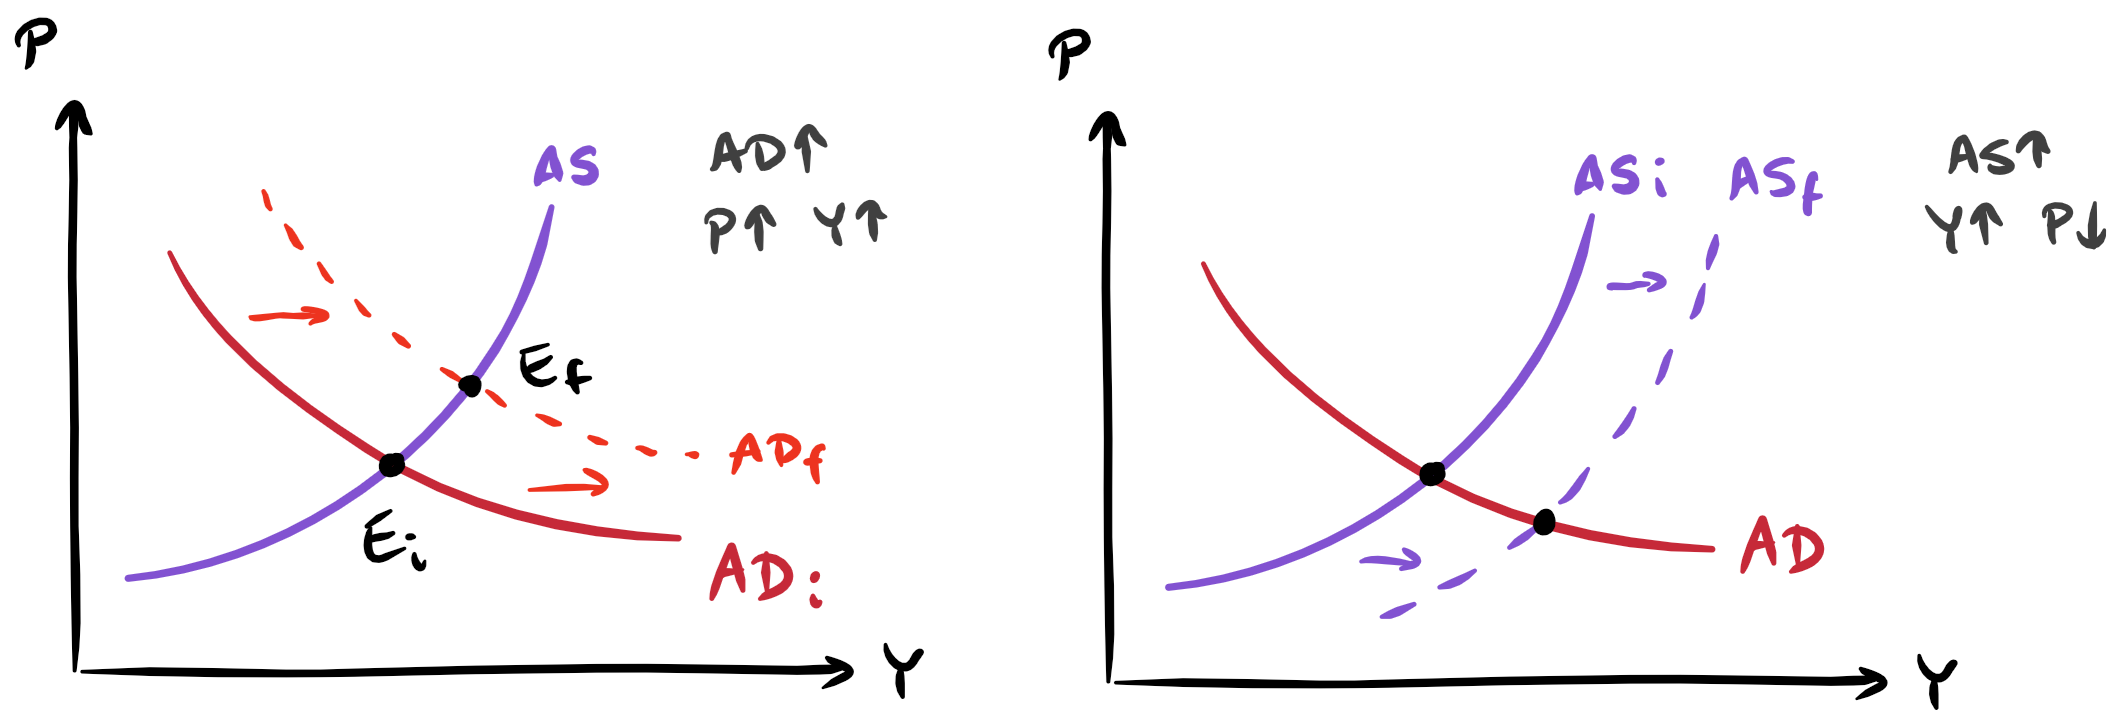
\includegraphics[width=110mm]{Img/23-4.png}
\caption{Equilibrium point of AS and AD Curve}
\end{figure}

When output is low, firms have excess capacity to fill, so a small increase in unit price mobilizes a great deal more output. Then gradually the effects diminish to almost nothing. 

\paragraph{Shifts in AS}

\begin{enumerate}

\item Decrease in factor prices shifts AS down and to right

\item Improvement in technology decreases input costs so AS shifts down and to right

\end{enumerate}

\subsection{Macroeconomic Equilibrium}

Occurs at  the combination of real GDP and price level where AS and AD intersect. 

The amount suppliers want to produce equals the amount households want to buy. Otherwise there would be shortages and surpluses. 

\subsubsection{Changes in Macroeconomic Equilibrium}

\paragraph{AD Shocks}

A shift in AD is called an aggregate demand shock. If it shifts rightward, it increases AD which means equilibrium GDP increases, so it's called a positive shock. If it shifts leftward, it decreases AD which decreases equilibrium GDP, so it is a negative shock.

AD shocks cause the price level and the real GDP to change in same direction. Cross arms and move left arm.

The multiplier measures the shift in horizontal movement if price level remains constant, so the multiplier is smaller when he AS curve is positively sloped.

\paragraph{AS Shocks}

Similarly, shifts in the AS curve cause positive and negative shocks. 

AS shocks cause the price level and the real GDP to change in opposite directions.


\section{Adjustment Process (Short-Run to Long-Run)}

The adjustment process evolves the short-run equilibrium to the long-run equilibrium. Let's talk about the key assumptions in each stage. 

\begin{enumerate}

\item \textbf{Short Run}

Factor prices are assumed to be exogenous. So they can change, but any changes are external to the model. Technology and factor supplies are also assumed to be constant, and so potential output $Y^*$ is constant. 

\item \textbf{Adjustment of Factor Prices}

In the adjustment process, which we will explore in more detail momentarily. The Factor prices are assumed to adjust in response to output gaps. Technology and factor supplies are similarly assumed to be constant, so $Y^*$ is constant. 

Essentially, we will examine how the effects of shocks and policies different between the short and long runs. $AD$ and $AS$ shocks have no long-run effect on GDP, and in the adjustment process $Y$ always returns to $Y^*$.

\item \textbf{Long Run}

In the long run, factor prices are fully adjustable in response to output gaps, so $Y$ always returns to $Y^*$. Technology and factor supplies are also assumed to change, such that $Y^*$ can grow.

\end{enumerate}


In summary, here is a table of there three stages.

\begin{table}[ht]
  \footnotesize
  \centering
  \caption{Short-Run, Adjustment Process, and Long-Run Assumptions}
  \begin{tabular}{
  		>{}m{0.6in} 
  		>{}m{1.1in} 
  		>{}m{1.1in}
  		>{}m{1.3in}  		  		
  		}
    \toprule
    \textbf{} & \textbf{Short Run} & \textbf{Adjustment Process} & \textbf{Long Run} \\ 
    \toprule
	 Assumptions 	& Factor $P$ exo. 		& Factor $P$ flexible 	& Factor $P$ endo. \\
	       		 	& Technology exo. 		& Technology exo. 		& Technology changing  \\
	       			& Factor supplies exo. 	& Factor supplies exo. 	& Factor supplies changing  \\
	       			& $Y^*$ exo. 			& $Y^*$ exo. 			& $Y^*$ changing  \\
	\midrule
	What Happens	& $Y$ determined by AS and AD	&	$Y$ moves to $Y^*$	&	$Y^*$ grows \\
	\midrule
	Why We Study	& $AD$ and $AS$ shocks effect on $Y$	&	See how gaps are closed	&	Understand long-run economic growth \\	
	\bottomrule

  \end{tabular}
\end{table}

\subsection{Output Gaps}

Real GDP is determined in the short run by the intersection of $AD$ and $AS$ curves. Potential output is assumed to be constant, so $Y^*$ is a vertical line. 

Following any aggregate demand or supply shock. The adjustment process describes the process by which $Y$ always returns to $Y^*$. Potential output can be described as an anchor that real GDP \textit{automatically} follows. 

\subsubsection{Inflationary Gap}

When $Y > Y^*$, there is pressure for factor prices to rise because when producing beyond capacity, inputs are in strong demand. This includes labour, so there will be labour shortages and so wages will rise. 

In response to having to pay more for inputs, firms will increase the prices of their products. So the $AS$ curve will shift up, so real GDP will decrease back to $Y = Y^*$. 

Additionally, the increase $AS$ temporarily increases the price level $P$, which is why it's called inflationary.

\begin{equation}
\begin{split}
Y < Y^*  \ & \ \Rightarrow \ Low\ demand\ for\ inputs  \\
 &\ \Rightarrow \ Wages\ \downarrow  \\
 &\ \Rightarrow \ Input\ costs\ \downarrow  \\
 &\ \Rightarrow \ Prices\ \downarrow  \\
 &\ \Rightarrow \ AS\ \downarrow  \\ 
 &\ \Rightarrow \ GDP\ \uparrow \ P\ \downarrow \\  
\end{split}
\end{equation}
\myequations{Adjustment Process for Inflationary Gap}


\subsubsection{Recessionary Gap}

When $Y < Y^*$, there is pressure for factor prices to fall because when producing under capacity, inputs will be in lower demand than normal. So there will probably be labour surpluses and unemployment, so wages will decrease. 

Again, now that firms unit costs are lower, they will decrease the prices of their products. So $AS$ curve shifts down, and real GDP increases back to $Y = Y^*$. 

\begin{figure}[ht!]
\centering
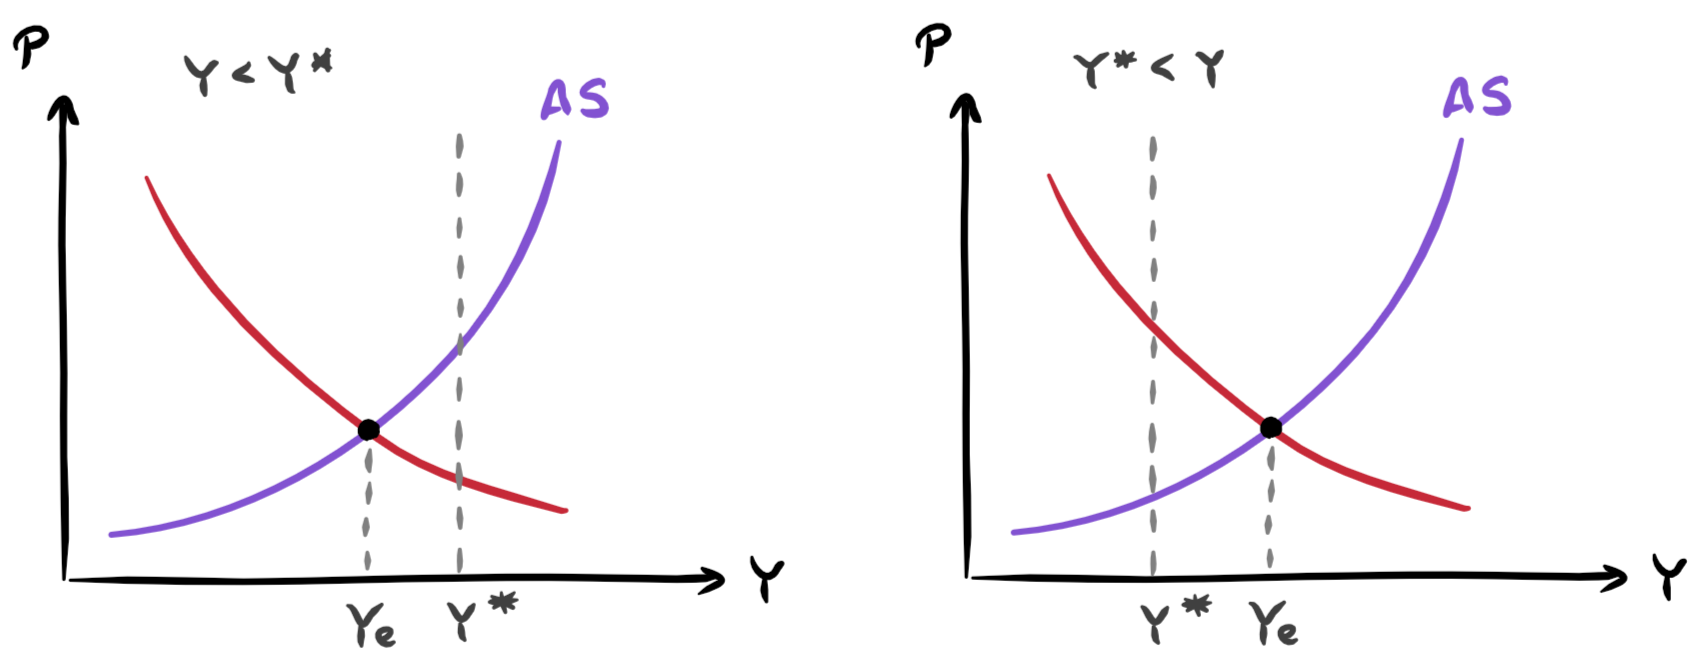
\includegraphics[width=110mm]{Img/24-1.png}
\caption{Output Gaps in the Short Run}
\end{figure}

Note that it takes much longer for wages to fall than for wages to rise, this is called \textbf{downward wage stickiness}. People are quick to accept wage increases, but it is much more challenging to reduce wages in short periods. 

For this reason, the adjustment process takes much longer for recessionary gaps than inflationary gaps. Inflationary gaps can be closed easily, but recessionary gaps are often described as \textit{languishing}. 

\begin{equation}
\begin{split}
Y > Y^*  \ & \ \Rightarrow \ High\ demand\ for\ inputs  \\
 &\ \Rightarrow \ Wages\ \uparrow  \\
 &\ \Rightarrow \ Input\ costs\ \uparrow  \\
 &\ \Rightarrow \ Prices\ \uparrow  \\
 &\ \Rightarrow \ AS\ \uparrow  \\ 
 &\ \Rightarrow \ GDP\ \downarrow \ P\ \uparrow \\  
\end{split}
\end{equation}
\myequations{Adjustment Process for Inflationary Gap}


\subsubsection{The Phillips Curve}

The Phillips curve is the inverse relationship of rate of change of wages and unemployment. To fight inflation it often requires unemployment, and to fight unemployment it often requires inflation. 

\subsection{AD and AS Shocks}

\subsubsection{Expansionary AD Shocks}

Suppose we start at $Y = Y^*$. Then there is a positive AD shock. This increases GDP and increases the price level, $P$. After this happens, $Y > Y^*$, so there is an inflationary gap. 

\begin{figure}[ht!]
\centering
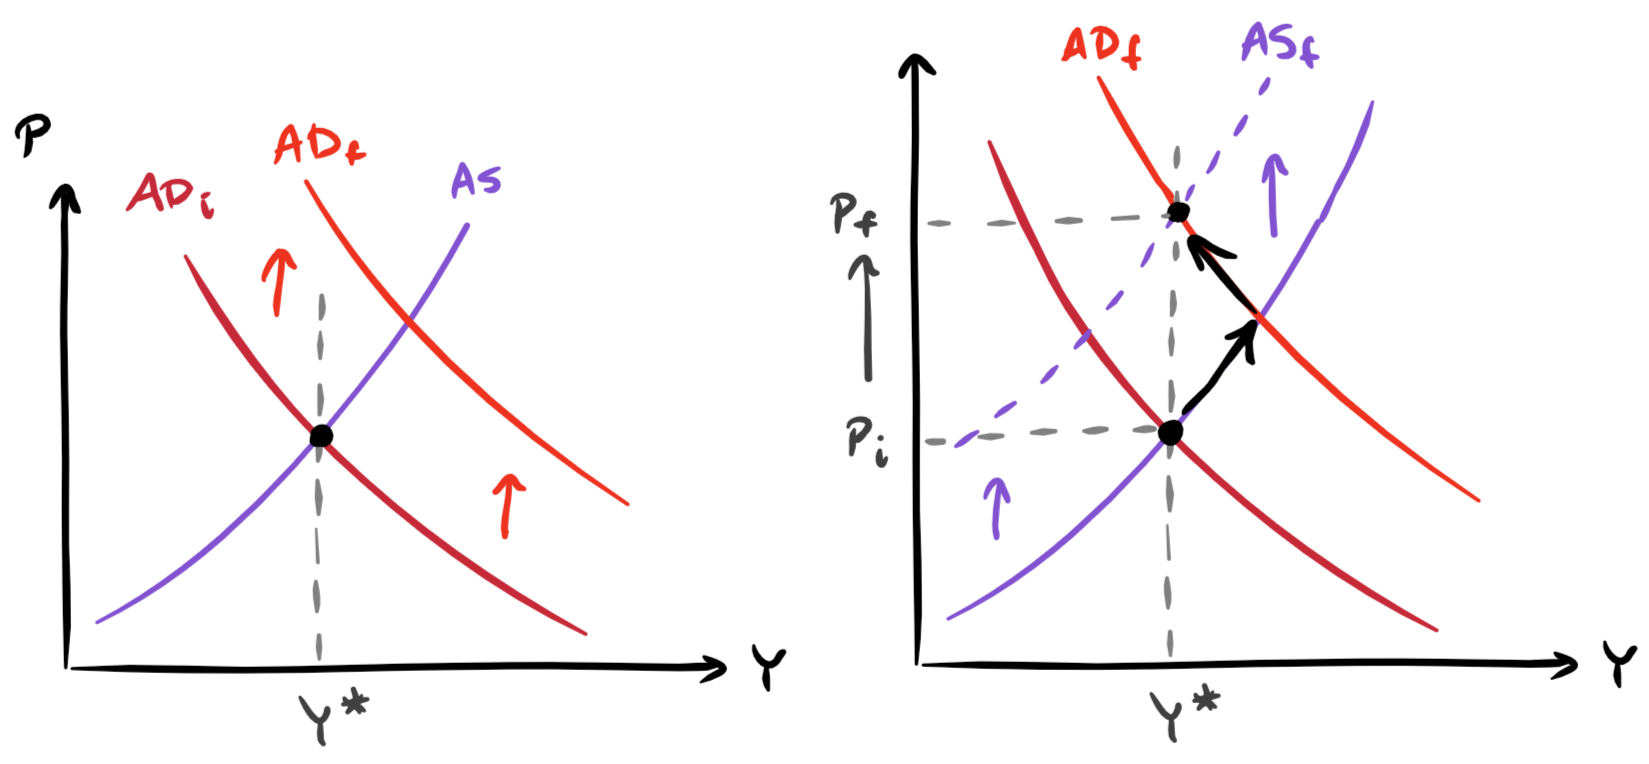
\includegraphics[width=110mm]{Img/24-2.png}
\caption{Adjustment Process to Positive AD Shock}
\end{figure}


In response to the inflationary gap, through the adjustment process discussed above, $Y$ decreases back to $Y^*$, but $P$ increases even further. So an expansionary $AD$ shock increases $P$. 

\subsubsection{Contractionary AD Shock}

Suppose we start at $Y = Y^*$. Then there is a negative AD shock. This reduces GDP and reduces the price level, $P$. After this happens, $Y < Y^*$, so there is an recessionary gap. 

\begin{figure}[ht!]
\centering
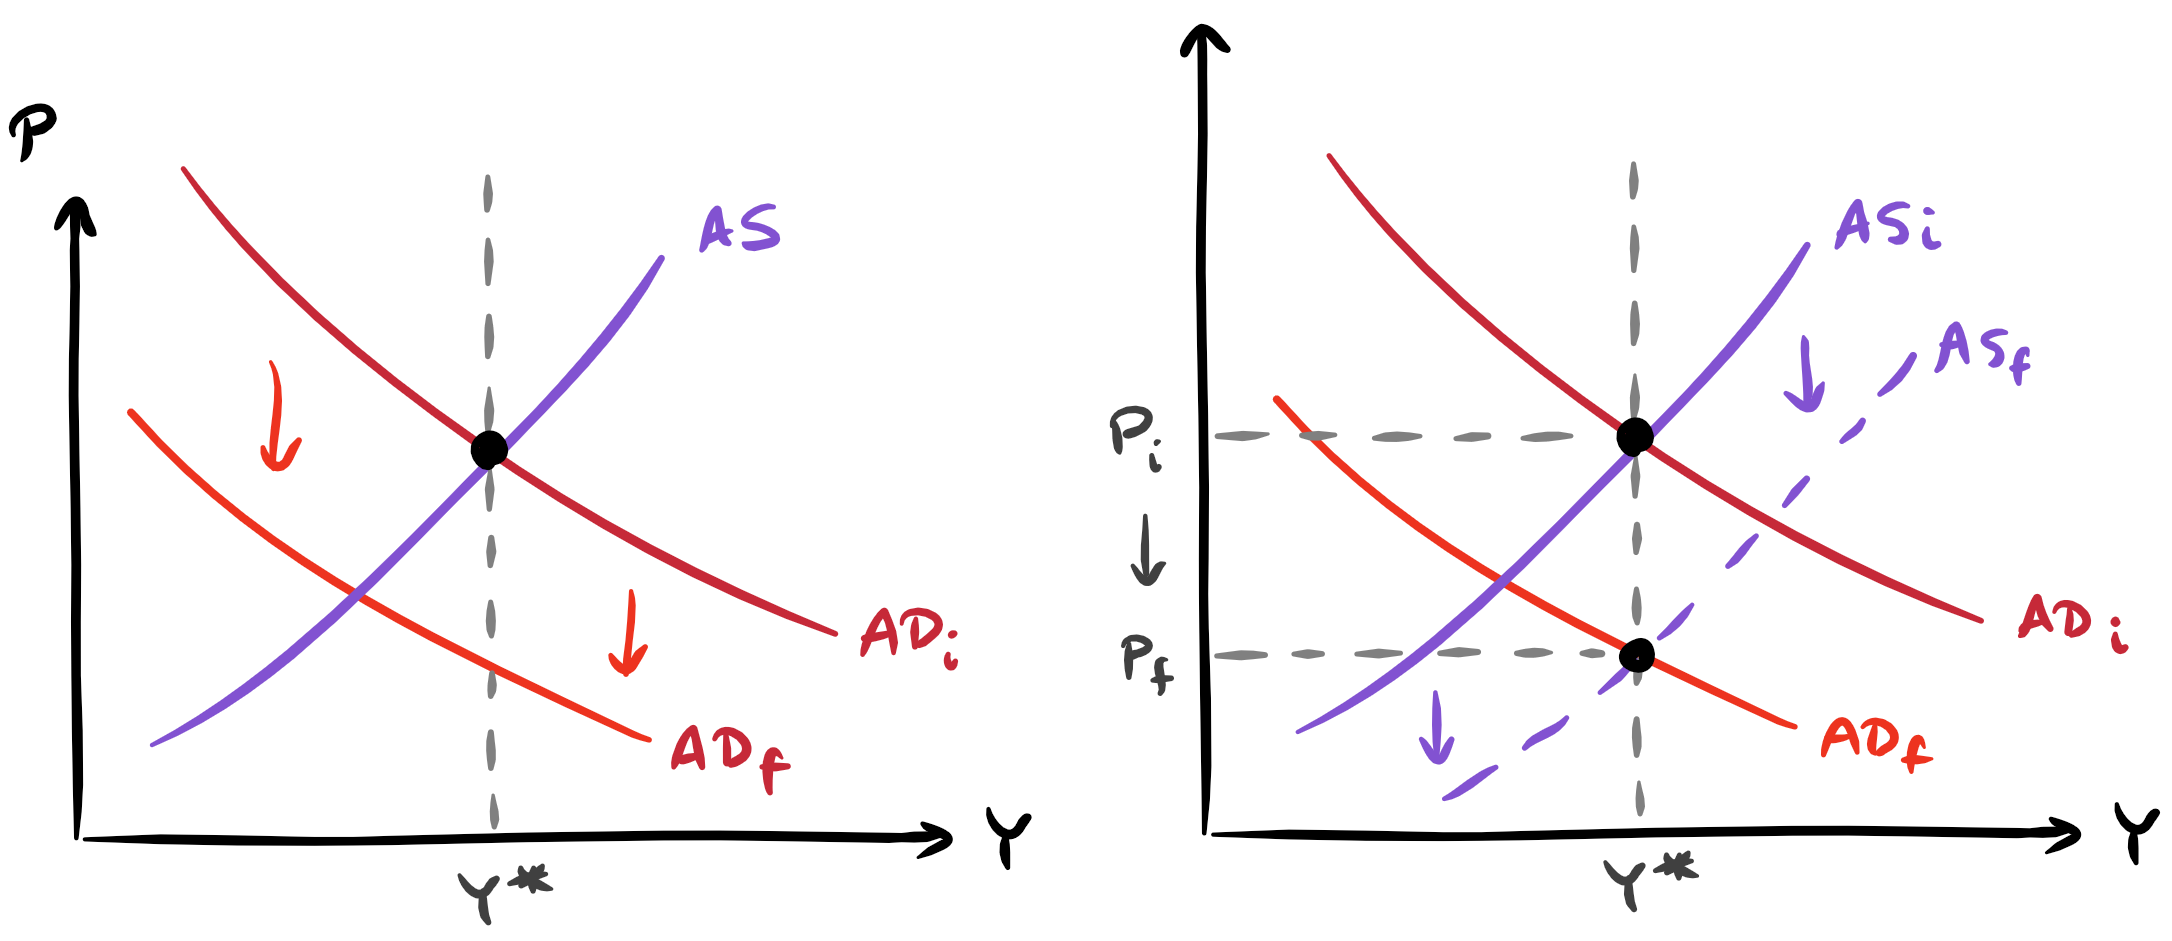
\includegraphics[width=110mm]{Img/24-3.png}
\caption{Adjustment Process to Negative AD Shock}
\end{figure}

In response to the recessionary gap, through the adjustment process discussed above, $Y$ increases back to $Y^*$, but $P$ decreases even further. So a contractionary $AD$ shock just decreases $P$. 

Recall that due to sticky wages, these processes are not completely symmetrical. An inflationary gap disappears faster than a recessionary gap, so a negative AD shock has a longer effect.

\subsubsection{AS Shocks}

With both positive and negative AS shocks, unlike AD shocks, when AS moves it changes both $Y$ and $P$ in the same direction. So by the time the recessionary gap or the inflationary gap has opened and then closed, the price level returns to the same initial level. 

\begin{figure}[ht!]
\centering
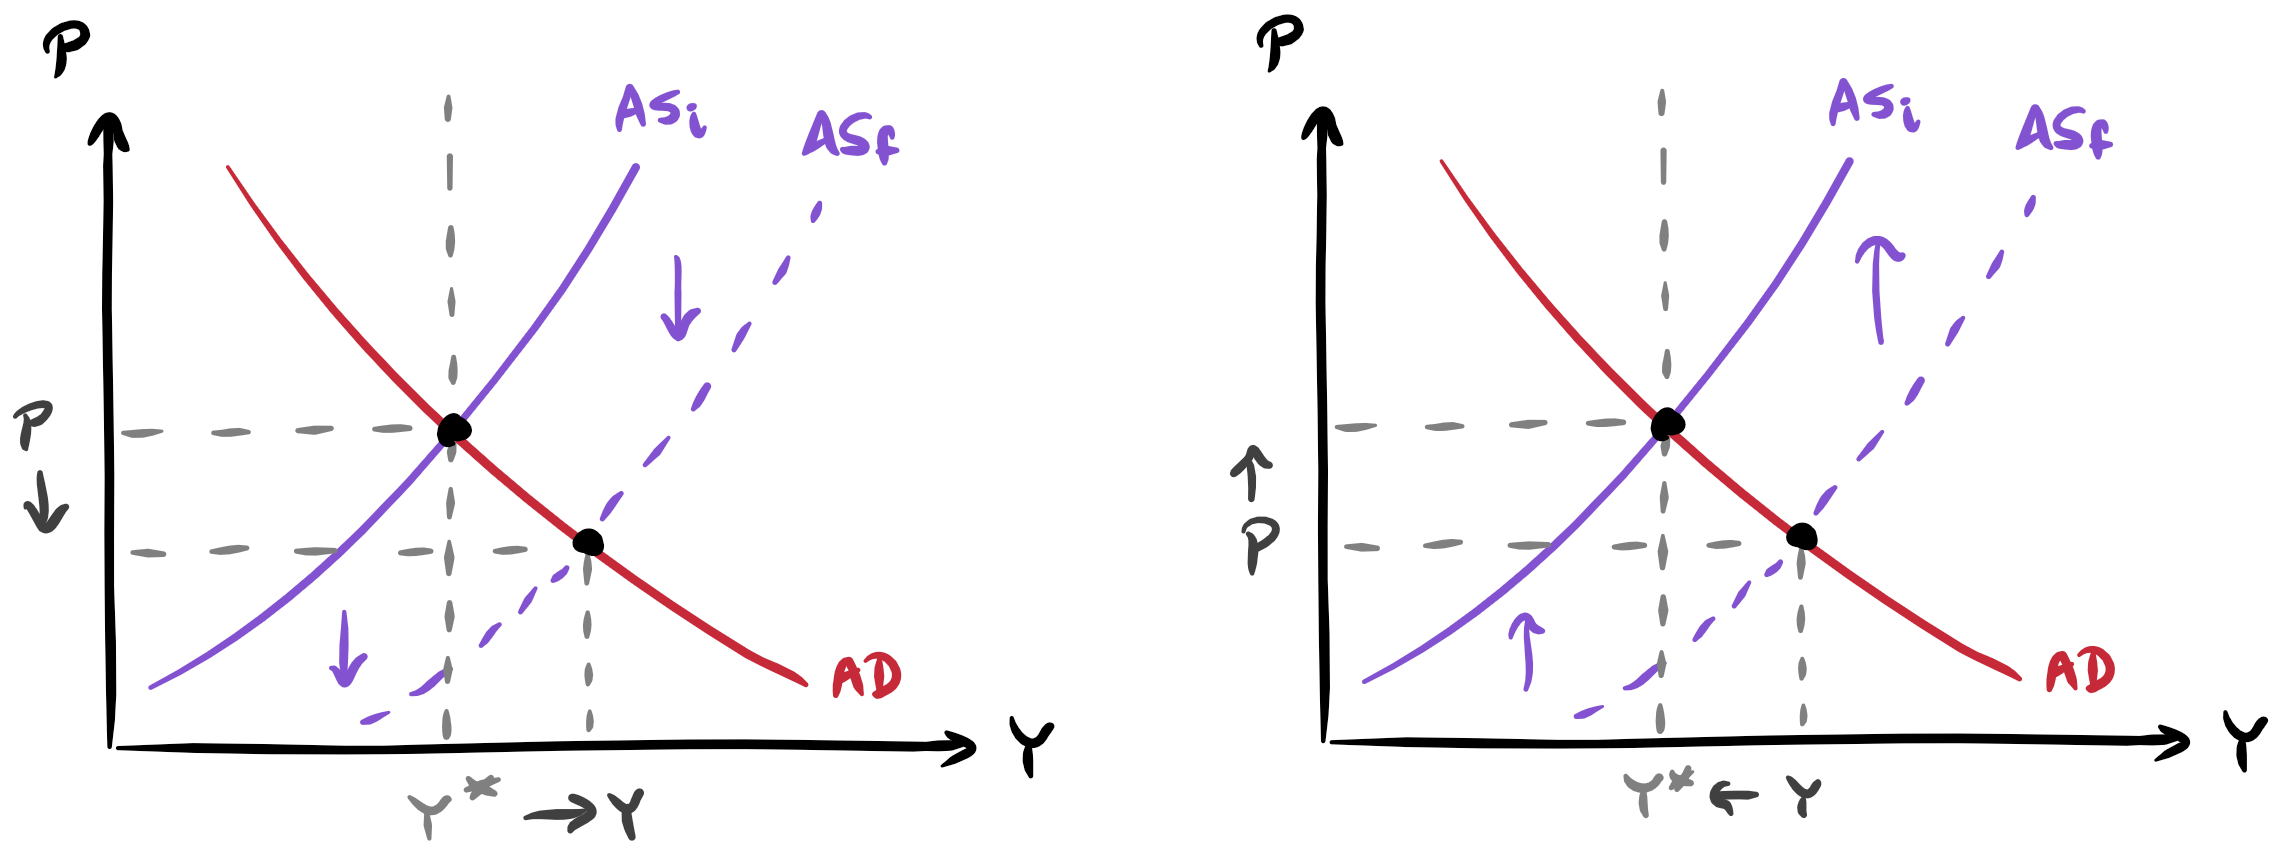
\includegraphics[width=110mm]{Img/24-4.png}
\caption{Adjustment Process to Negative AS Shock}
\end{figure}


\subsubsection{Long-Run Equilibrium}

The economy is said to be in long run equilibrium when when the adjustment process has completed. In this case, the only way GDP can change is if $Y^*$ increases, and $AS=Y^*$, a vertical line. As it increases, the price level diminishes, and if it decreases, the price level rises.

%fig 24-5%

%fig 26-17 in book

\subsection{Fiscal Stabilization Policy}

The government can change taxation and government spending to push real GDP back to potential output in cases where recessionary gaps or inflationary gaps persist. 


\subsubsection{Closing a Recessionary Gap}

In cases of recessionary gaps where sticky prices keep the gap from closing, the government can use a reduction in $T$ or an increase in $G$ to increase $AE$ and shift $AD$ to the right. This can shorten an otherwise long recession. 

If this persists too long though it can overshoot and cause an inflationary gap. 

\subsubsection{Closing an Inflationary Gap}

By increasing $T$ or decreasing $G$, the government can shift $AD$ to the left. The benefit of this is that if left to close automatically, the price level would rise and there would be inflation. 

Using contractionary fiscal policy, you can avoid that inflation. Similarly as above however, there is the risk of overshoot and opening up a recessionary gap. 

\subsection{The Paradox of Thrift}

In the short-run, an increase in savings reduces real GDP. In the long-run, an increase in savings means that more financial capital is available for investment, and so real GDP increases. 

The \textbf{paradox of thrift} is that what's good for individuals can be bad for economies as a whole, and what's good in the short-run can be bad in the long-run. 

\subsection{Automatic Stabilizers}

All of the policies discussed above are called \textbf{discretionary policies} because they require an overt decision by the government. However, \textbf{automatic stabilizers} can dampen the effects of shocks without active decisions. 

The most common automatic stabilizer is the tax-and-transfer system. Consider a positive AD shock, which would increase real GDP and reduce $P$. As GDP increases, tax revenues increase and the government makes less transfer payments, so $T$ increases. This automatically pushes GDP back down, or at least reduces the effects of the shock. 

\begin{equation}
\begin{split}
Y > Y^*  \ 	&\ \Rightarrow \ Tax\ revenues \uparrow \ Transfers \downarrow  \\
 			&\ \Rightarrow \ T \uparrow  \\
 			&\ \Rightarrow \ Y \downarrow  \\
\end{split}
\end{equation}
\myequations{Automatic Stabilizers with Tax-and-Transfer System}

\subsection{Limitations of Discretionary Fiscal Policy}

\subsubsection{Decision/Execution Lags}

\textbf{Decision lags} are the period of time between the government being able to recognize a problem like an output gap, and then making a decision about what to do about it -- for instance, what to increase spending on, or whose taxes to cut and by how much. 

\textbf{Execution lags} are the period of time between when the policy is enacted and when its effects can be felt. It is worthwhile to note that when adjusting $G$, the execution lag is much longer than when adjusting $T$. The time it takes for new programs or infrastructure to be created takes much longer than changing taxes, which can be felt almost immediately.

\subsubsection{Temporary vs. Permanent Tax Changes}

Temporary tax changes are typically less effective than permanent tax changes, because individuals will not fully adjust their spending habits if they know things will revert back to they way they used to be. 

The more forward-looking households are, the smaller the effects of temporary changes in taxes are. 

\subsection{Fiscal Policy effect on Growth}

So as we know $Y$ will always return to $Y^*$ in the short-run, and we assume $Y^*$ is constant in the short-run. We will now investigate the effects fiscal policy may have on increasing $Y^*$ in the long-run. 

\subsubsection{Increase in Government Purchases}

As we now know, an increase in $G$ will shift $AD$ to the right, increasing real GDP beyond $Y^*$ in the short run. So factor prices will increase, so wages will increase, so prices will increase, so $AS$ will increase, and finally $Y$ will return to $Y^*$ but $P$ levels will have increased. 

Let's now consider the effects that in increase in $G$ may have on $Y^*$. 

Even though $Y = C + I + G + NX$ will return to $Y^*$, since $G$ has increased, composition of $Y^*$ has changed. This means that there must be some fall in $G + I + NX$. In which case, we say that government purchases have \textbf{crowded out} private expenditures and potentially capital investment. When private investment is crowded out, this can reduce the future growth rate of $Y^*$.

However, if government purchases are in public infrastructure that increases private-sector productivity and production, such as highways, bridges, ports, and electrical lines, then $Y^*$ can also rise and the crowding out effect will be minimized. 

\subsubsection{Reductions in Taxes}

Reductions in $T$ increase $C$ and $I$, which shifts $AD$ to the right, increasing real GDP. Again through the adjustment process, wages will increase to $Y$ will return to $Y^*$. 

However, this means less money in the hands of the public sector and more in the hands of the private sector, but if capital investment is increased this can increase the growth rate of $Y^*$. 

\subsubsection{Supply-side Economics (Reaganomics)}

In the 1980s, Reagan and Thatcher tried another method entirely. The idea of \textbf{supply-side economics} was that extensive reductions in tax rates would increase economic activity and increase $Y^*$ so much, that the amount of tax revenue lost by reducing taxes would be offset by the increase in revenue from the new economic activity. 

Instead of returning $Y$ to $Y^*$ in an inflationary gap, they aimed to close the gap by increasing $Y^*$. This means inflationary gaps can be closed without moving $AD$. It definitely worked to increase economic activity, but it's a stretch to say it actually increased government tax revenue. 


\section{Long-Run Economic Growth}

Economic growth is the most power tool for long-term increases in human living standards. Real GDP is the total measure of economic activity, but average material living standards are usually measured in terms of real GDP per capita. The main reason for this increase over time is due to productivity -- typically measured as real GDP per employed worker. 


\subsection{Benefits of Economic Growth}

Long run growth has two main benefits...

\begin{enumerate}

\item \textbf{Rising average living standards} -- Increases in real GDP per capita are typically dispersed to the population through increases in the average income. 

Higher incomes allow families to buy important amentities and allow saving ffor the future. It also tends to shift consumption away from goods such as TVs, to services such as vacations and dining out. 

\item \textbf{Addressing poverty and income inequality} -- Even though the average income is increasing, it has be disproportionally dispersed to the highest earners in an economy.  Unemployed people are especially hurt by this, because increasing average income simply increases everyone's wealth around them. 

A high growth rate however makes poverty alleviation and income redistribution easier politically. Without a growing economy, redistribution of income requires taking from someone and giving to someone else, which is politically sensitive and also effectively reduces someone's living standards. However, with economic growth, income can be redistributed without reducing someone's living standards, rather when there is growth, everyone's incomes can rise but it can be disproportionally allocated to lower-earners. 

\end{enumerate}


\subsection{Costs of Economic Growth}

\begin{enumerate}

\item \textbf{Forgone consumption} -- Increases in real GDP per capita is often the result of investment expenditure. However, this investment means current consumption is being sacrificed by the current generation consumers. Economic growth promises more goods and services in the future, at the expense of lower consumption now. 

\item \textbf{Social costs} -- Economic growth means old firms, capital, and labourers are overtaken by new firms, capital, and labourers. High economic growth means that within a generation workers can find their skills rendered obsolete, which has high social costs.

\end{enumerate}

\subsection{Sources of Economic Growth}

\begin{enumerate}

\item \textbf{Growth in the labour force}

\item \textbf{Growth in human capital} -- the quality of the labour force, via education, experience, or training

\item \textbf{Growth in physical capital} -- factories, equipment, communications, etc. We also include improvements in the quality of the capital here. 

\item \textbf{Technological improvements}


\end{enumerate}

\subsection{Theories of Economic Growth}

Different theories emphasize different aspects of the sources of economic growth. Common across them is that in the long run, we assume there are no output gaps, that is, real GDP equals potential output $Y = Y^*$. 

\subsubsection{Long-Run Economic Growth Model}

At the equilibrium level of real GDP, desired savings equals desired investment, $S = I$. Additionally, in the long-run the interest rate $i$ is an endogenous variable, and its value is determined by the equilibrium point where total savings equals investment.

%fig 26-2 / 26-3%

\begin{equation}
\begin{split}
Private\ savings  	&\ = Y^* - T - C \\
Public\ savings  	&\ = T - G \\
\Rightarrow \ National\ savings 	&\ = Y^* - C - G \\
\end{split}
\end{equation}
\myequations{Public, private, and national savings}

When the national savings increases so the $NS$ curve shifts right, there is an excess supply of financial capital, so its not risky to lend out, so there is a decrease in the interest rate.

On the otherhand, when national savings reduce, there is a shortage in the supply of financial capital, so there is an increase in the interest rate. 

\textit{So more savings reduces interest rate, which results in more investment. A higher equilibrium level of investment leads to a higher future growth rate of potential output.} 

\subsubsection{Neoclassical Growth Model}

The \textbf{neoclassical growth model} says that labour, capital, human capital, and the state of technology form the \textbf{aggregate production function}, which relates the economy's total output to  the total input factors. Note however, that technology is exogenous. 

$$GDP = F_T (L, K, H)$$

Characteristics of the neoclassical growth model

\begin{enumerate}

\item \textbf{Subject to diminishing marginal returns} when any one input factor is increased by itself.

This means that increases in the population (labour) for instance will increase real GDP, gradually it will actually reduce real GDP per capita, reducing living standards.

Similarly, increases in capital will increase material living standards, but the improvements because smaller with each increment.

\item \textbf{Subject to constant returns to  scale} when all inputs are increased in proportion

If labour and capital grow at the same rate, then real GDP will most certainly increase. However, because of constant returns real GDP per capita will remain the same -- there will be no increase in living standards.

\item \textbf{Assumes technology is exogenous} 

This is likely the reason that the theory cannot seem to reconcile the increasing living standards of the modern world. \textbf{Embodied technological change} is the process by which old capital is replaced by improved quality capital. This means the quantity of capital may seem constant, there is an increase in the productive capacity of the economy, increasing potential output even if labour and capital are constant.

Technological change was classically measured with the \textbf{Solow residual}, also called total factor productivity, which was the amount of economic growth that could not be accounted for by growth in labour or capital.

\end{enumerate}

\subsubsection{Modern Growth Model}

Modern growth theories have expanded upon the neoclassical growth model by modifying two assumptions.

\begin{enumerate}

\item \textbf{Technology is endogenous} -- technological change is responsive to the economic system. Increases in technology are often undertaken by firms in search of profits. 

\item \textbf{Increasing marginal returns} -- new increments of investment are often more productive than previous increments. Initial stages of investment can be marginally more productive, but through a learning curve, investment can be worth more and more. 

As a result, followers in an industry can have a great economic advantage to pioneers of investment. Partly because avoiding the learning curve costs, but also because consumers can be slow to adopt new technologies. 

\end{enumerate}



\section{Money and Banking}

\subsection{Definition of Money}

Money is...

\begin{enumerate}

\item \textbf{a medium of exchange} -- recognizable, divisible, durable, hard to counterfeit, facilitates trade

\item \textbf{a store of wealth} -- spending and earning don't have to be synchronized, must have stable value

\item \textbf{a unit of account} -- common denominator of worth, two units of \$1 are equal to \$2, can be used for accounting without physical existence

\end{enumerate}

\subsection{History of Money}

\subsubsection{Metallic Money}

All sorts of things have been used as money, but metals like gold and silver were the most successful. They were easily recognizable, divisible, and did not wear out. Before the invention of coins, people had to carry it around in bulk and weigh it on scales. 

Coins eliminated this need by creating fixed units, however this needed an authority to guarantee the value. So monarchs would stamp the coin with their seal and the coin would then be accepted at "face value". This led to edge clipping and debasing coins by mixing in cheap metals like nickel. \textbf{Gresham's Law} states that money that's been debased usually stays in circulation, whereas "good" money tends to hoarded. 

\subsubsection{Backed Paper Money}

Goldsmiths had very secure safes. So people began leaving their gold with them, and in exchange the goldsmith would give them a receipt, stating the goldsmith would return their gold on demand. 

Eventually, people began to trade the receipts instead gold, this was basically the first paper money. Then commercial banks began to do this with all sorts of proprietary "bank notes" instead of the goldsmiths. This is what's known as \textbf{backed money}, money that is backed up by gold and is convertible to gold upon demand. 

\subsubsection{Fractionally-Backed Money}

Banks soon realized that not many people will come in and want to convert their money to gold upon demand, and rarely will everyone do it at once. So instead of storing all the gold in the bank, they could keep, say 20\% of it in reserve and begin loaning out the rest with interest to make some profit. 

So the banks were issuing more bank notes than they had to back it up. If some people wanted to convert it to gold, they could do so, but not everyone all at once. A risky bank could invest more money, but run at low reserves, whereas a more cautious bank would keep higher reserves. 

This is what banks continue to do to this day.

\subsubsection{Fiat Money}

Eventually governments stepped in and the central bank became the only bank to issue currency. Originally the central banks were similarly backed by gold, known as the \textbf{gold standard}, but around WWII most countries ditched this in favour of \textbf{fiat money} -- money that isn't backed by anything, we just use it because the government issues it and everyone have faith in it. 

This is known as \textbf{legal tender} -- money that legally must be accepted to repay a debt, otherwise the debt is forgiven. 

\subsubsection{Deposit Money}

Now people have gone a step further, and we deposit our fiat money in bank accounts for safekeeping. These deposits can be used to make transactions even though they're just electronic entities.

The value of the deposit money now exceeds the value of cash currency. Like the banks before, modern banks have issued more IOUs (deposits) than they have cash in reserve. Like before with gold, banks run on a \textbf{fractional-reserve system} -- at any given time if people choose to withdraw all the cash they have deposited in the bank, the bank's in trouble. 

\subsection{The Banking System}

\subsubsection{The Central Bank}

The \textbf{central bank} is the government-owned and government-operated institution in a country. However, the Bank of Canada is not responsible to parliament and has autonomy to operate monetary policy independent of day-to-day political influence. This is known as \textbf{joint responsibility}.  

The responsibilities of the central bank are as follows

\begin{enumerate}

\item \textbf{Bank for Commercial Banks} -- If banks run out of their reserves and need to borrow money, they can do so from the central bank. Different commercial banks also use the central bank to transfer money to and from each other. 

\item \textbf{Bank for the Government} -- The government bank account is in the central bank, from which they can make deposits and write checks. When the government requires more money than it collects in taxes, it borrows by selling treasury bills or government bonds to the central bank.

\item \textbf{Regulate Money Supply} -- They print money. This is only done as a reaction in Canada. 

\item \textbf{Support Financial Markets} -- When banks are about to go under, the central bank bails them out to prevent panic and bank failures. 

\end{enumerate}

\subsubsection{Commercial Banks}

Commercial banks are privately owned, profit-seeking institutions. They provide services like checks and debit cards to make easy transactions, they also provide convenient savings accounts to earn small but guaranteed interest, and financial advisement. 

With peoples' savings, they invest in government securities, make loans to households and firms, and divide loans into small pieces and repackage them into \textbf{securities}. 

Credit is the lifeblood of the modern economy. For instance, wages for workers and production materials have to be paid well before the revenue for a new product is earned. Firms have to fund their capital investments with the borrowed money, and when firms have no access to credit, many businesses would grind to a halt. 

The main \textbf{asset} of commercial banks is stakes in securities and loans. Their main \textbf{liability} are their deposits, which they will have to repay on request. They therefore keep a percentage of money in the bank that they do not lend out, called a \textbf{reserve-ratio}. 

\subsection{Money Creation}


\subsubsection{Expansion of Money}

Consider someone takes \$1000 cash out from under their bed and deposits it in the bank, and assume the reserve ratio (RR) is 20\%.  The bank would then lend out \$800 to the world. Then these people would go out and buy \$800 worth of stuff, so the \$800 would end up in someone's bank account. At which point, this other bank would lend out  \$800(80\%) = \$640, which would then be spent and so on and so forth. 

This process effectively creates deposit money. In the end, the increase in the supply of money is dependent on the reserve ratio. This is called the multiple expansion of deposits.

\begin{equation}
\Delta M = \Delta D \times \frac{1}{RR}
\end{equation}
\myequations{Money Multiplier}

\subsubsection{Cash Drain}

Above we assumed that people deposit all of the money they don't spend. However, in real life people hold onto a fraction of their bank deposits in cash. This is called cash drain, and it is quantified using the currency ratio (CR). We assumed CR was zero above, but now it influences our expansion of money formula.

\begin{equation}
\Delta M = \Delta D \times \frac{1}{CR + RR}
\end{equation}
\myequations{Money Multiplier with Cash Drain}

Realistic values for these in Canada are $RR = 1\%$ and $CR = 5\%$, so in the previous example concerning a new deposit of \$1000. This would actually translate to \$16,666. So as you can see, with such a small reserve ratio, small changes in deposits amount to huge changes in the money supply.

\subsection{Money Supply, $M$}

There are multiple definitions of the money supply, but mainly you can consider it as the sum of currency in circulation and bank deposits at chartered banks that can be easily transferable, \textbf{demand deposits} (think checking account).

\begin{equation}
\begin{split}
M1 & =  Currency + Demand\ deposits \\
\end{split}
\end{equation}
\myequations{Money Supply}

There is also $M2$ which include notice deposits (think savings account), $M2+$ which includes deposits at other financial institutions, and $M2++$ which includes savings bonds and all other mutual funds. The M1 definition is based emphasizing the medium of exchange, the latter merely include anything considered a store of wealth. 

\subsubsection{Other Types of Money}

\textbf{Near money} are assets that can easily be converted into money and are a store of wealth, but are a poor medium of exchange -- think term deposits. On the otherhand, \textbf{money substitutes} are things that are a good medium of exchange, but are a poor store of wealth -- think credit cards.

\section{Monetary Theory}

We will group wealth into two categories, "money" and "bonds". Consider money as anything that serves as a medium of exchange -- including cash and deposits checking accounts, and bonds as other forms of wealth -- savings accounts and capital assets. 

This is important because we must distinguish between interest-earning assets and non-interest-earning assets.

\subsection{Bonds}

\subsubsection{Present Value and Interest Rates}

A bond is an asset that promises to make one or more fixed payments at fixed intervals in the future. The \textbf{present value (PV)} of an asset refers to the current value of the expected future payments using the \textit{current rate of interest}. 

\begin{equation}
PV = \frac{FV}{(1+i)^t}
\end{equation}
\myequations{Present Value}

Typically they make fixed "coupon" payments every year, then pay back the original "face value" of the bond at the end of the term of the loan. The coupon payments are based on the current interest rate at the time the bond was purchased. 

So if the interest rate increases afterward, the bond is worth less -- it has a lower present value. On the otherhand, if the interest rate drops, the bond is worth more -- it has a higher present value. A reduction in bond prices means an increase in bond yields. 

*********

\begin{equation}
i \uparrow \ Bond\ price \downarrow \ Bond\ yield \uparrow
\end{equation}

The only risk of bonds is that the bond issuer will not be able to make the payments, for instance, if the company goes bankrupt. For government bonds, this is quite unlikely. 

The yield of a bond can change because of a change in the perceived risk of the bond. An increase in the riskiness of a bond results in a lower expected present value, and thus a decline in the the bond's price, and an increase in the bond yield.

\begin{equation}
risk \uparrow \ Bond\ price \downarrow \ Bond\ yield \uparrow
\end{equation}

\subsection{Money Demand, $L$}

People have to choose what ratio of money to bonds they want to hold at any given time. If you hold more money, you hold fewer bonds, and vice-versa. The amount of money that everyone collectively holds at any given time is called the \textbf{demand for money}. The willingness to hold money over bonds is called the \textbf{liquidity preference function}, $L$. 

\subsubsection{Reasons for Money Demand}

\begin{enumerate}

\item \textbf{Transactions demand} -- money kept to make routine transactions

\item \textbf{Precautionary demand} -- money kept in the event of an unexpected emergency

\item \textbf{Speculative demand} -- money kept typically by businesses in anticipation of increasing future interest rates, thus declines the the value of bond holdings

\end{enumerate}

\subsubsection{Determinants for Money Demand}


\begin{enumerate}

\item \textbf{Interest rate} -- the opportunity cost of holding money is the income that could have been earned on the interest of investing, so an increase in interest rate reduces the quantity of money, $ i \uparrow  \ L \downarrow $


\item \textbf{Real GDP} -- When real GDP is higher, people make more transactions, so an increase in GDP increases the quantity of money demanded,  $ Y \uparrow  \ L \uparrow $

\item \textbf{Price Level} -- When the price level is higher, people need more money in their pockets to conduct their regular transactions, so an increase in price level increases the quantity of money demanded, $ P \uparrow  \ L \uparrow $

\end{enumerate}


\subsection{Monetary Equilibrium}

The monetary equilibrium is the intersection of the supply of money curve $M$, and the demand for money curve $L$. The equilibrium occurs when the interest rate is such that $M = L$. 

%fig 28-2%

The supply curve, $M$, is independent of the interest rate, so it is a vertical line. The demand curve is a downward sloping line because when the interest rate falls, the quantity of money increases. 

\subsubsection{Monetary Transmission Mechanism}

There is a relationship between the demand and supply of money and aggregate demand. In essence, by changing the money supply we can shift aggregate expenditure, real GDP, in the short run. This is called the \textbf{monetary transmission mechanism}.

This occurs in three stages...

\begin{enumerate}

\item \textbf{Change in demand/money supply change the interest rate}

Suppose there is an increase in the money supply or a decrease in the money demanded. This creates an excess supply of money. 

So since everyone has extra money, everyone starts buying more bonds, and by supply and demand the price of bonds increases.

The increase in the price of bonds causes a decrease in the interest rate.

%fig 28-3%

\item \textbf{Change in the interest rate changes aggregate expenditure}

Continuing from above, suppose the interest rate decreases. This will lead to more investment expenditure (recall by this we mean investment in mortgages and cars and other things purchased on credit, not investment in accounts), so $I$ increases. Similarly, consumption expenditure $C$ increases. 

%fig 28-4%

On top of $I$ and $C$ increasing, we also get $NX$ increasing. This is because a decrease in interest rates means investors will sell Canadian bonds and buy foreign bonds instead. This means Canadian dollars will decrease in desirability relative to other currencies, so it depreciates in value. 

This means that Canadian goods are more cheap relative to foreign goods, so imports decrease and exports rise, thus $NX$ increases. This is the \textbf{open-economy modification}.

All of these changes shift aggregate expenditure up.

\item \textbf{Change in AE shift the AD curve}

A shift upward in the AE curved caused by something other than a change in price level leads to a rightward shift in the AD curve. 

So finally, this rightward shifts increases the short-run real GDP and the price level.

%fig 28-5%

\end{enumerate}

So that's quite a process but let's recap. 

\begin{equation}
\begin{split}
M \uparrow \ or \ L \downarrow \ & \ \Rightarrow \ Excess\ money  \\
 &\ \Rightarrow \ P_B \uparrow  \\
 &\ \Rightarrow \ i \downarrow  \\
 &\ \Rightarrow \ I \uparrow \ NX \uparrow  \\
 &\ \Rightarrow \ AE \uparrow  \\ 
 &\ \Rightarrow \ AD \rightarrow  \\  
 &\ \Rightarrow \ GDP \uparrow P \uparrow  \ (short\ run) \\   
\end{split}
\end{equation}
\myequations{Flow of Money Supply on GDP}

\subsubsection{Slope of AD Curve Revisited}

This is the main reason that the AD curve is downward sloping. A rise in the price level causes a rise in the demand for money, which shifts the $L$ curve to the right, increasing the interest rate. 

This increase in $i$ leads to a reduction in $I$ and thus $AE$. So in the end $P \downarrow \ AE \uparrow$, which is the negative slope we were talking about.

\section{Inflation}

\textbf{Inflation} is a rise in the average level of prices. It hasn't been a big deal in the last couple of decades, but historically it has been considered a serious problem. 

There are two kinds of inflation, anticipated inflation and unanticipated inflation. The former is healthy, but the latter is more troublesome.

One of the main problems with unanticipated inflation, is that businesses, investors, and consumers want to participate in a stable and predictable economy. It's difficult to make long-term plans in economies suffering from inflation, because there is so much uncertainty regarding the future of real wages, real interest rates, and relative prices. 

\subsection{Inflation in our Model}

As we have seen, AD and AS shocks influence the real GDP and also the price level. These shocks could push the price level up, causing temporary inflation, but the adjustment process would always bring the economy back to the equilibrium level of output and a stable price level.

Now we will see the effects of sustained, and accelerating inflation. 

\subsubsection{Wage Changes}

\paragraph{Wages Changes from Output Gaps}

Recall that increases in wages increased unit costs, driving up prices, and driving up the AS curve. Conversely, falling wages drops the AS curve, though this happens more slowly. 

At the equilibrium point, and the unemployment level is \textbf{NAIRU} -- the non-accelerating inflation rate of unemployment, $U^*$. NAIRU is not zero, even when output is at potential, because there will always be frictional and structural unemployment. 


\begin{enumerate}

\item $Y > Y^*$ results in excess demand for labour. $W \uparrow$ and $U < U^*$

\item $Y < Y^*$ results in surplus supply of labour. $W \downarrow$ and $U > U^*$

\item At equilibrium, wages are constant and the unemployment rate is equal to NAIRU

\end{enumerate}

\paragraph{Wage Changes from Expected Inflation}

Since employees and employers can look back at the rate of inflation in previous years, there are expectations about future inflation. So many employees have the bargaining power to expect a 2\% increase in nominal wages per year to match inflation.

However, say inflation is then only 1\% but nominal wages increase by 2\%, so real wages can increase even when there is no inflationary gap as long as people expect prices to rise. 

\subsubsection{Price Changes}

Upward shifts in the AS curve will cause prices to rise, so the forces pushing wages up will be \textbf{inflationary}. Downward shifts in the AS curve will cause prices to drop, so the forces pushing wages down will be \textbf{deflationary}.

Inflation caused by wage increases is the sum of three components: \textbf{output-gap inflation}, \textbf{expected inflation}, and \textbf{supply-shock inflation}.

\subsubsection{Constant Inflation}

Here we are assuming that output is at potential and there aren't any shocks. There are three requirements of constant inflation...

\begin{enumerate}

\item Expectations of inflation -- shifts $AS$ up

\item Expansionary monetary policy by the central bank -- shifts $AD$ up

\item The rate of monetary growth is equal to the expected rate of inflation -- $Y$ remains at $Y^*$

\end{enumerate}

When the central bank increases the money supply to cancel out the anticipated inflation, the bank is said to be \textbf{validating} the exceptions. 

%fig 30-2%

\subsection{Shocks and Policy Responses}

In many cases the inflationary  pressures are  created by AD or AS shocks. Here we assume that potential output isn't influenced by these shocks, but this isn't necessarily true in the long-run. 

\subsubsection{Demand Shocks}

When the AD curve shifts right and it opens up an inflationary gap, this is said to be \textbf{demand inflation}. There are two possible outcomes of this scenario, depending on if the central bank chooses to validate or not. 

\begin{enumerate}

\item \textbf{No monetary validation} -- Excess labour demand increases wages, which increases factor inputs, which increases AS, and the gap is closed at a higher price level

\item \textbf{Monetary validation} -- The bank could increase the money supply to sustain the inflationary gap in an attempt to keep operating at a higher GDP. This changes temporary inflation into sustained inflation.

\end{enumerate}

%fig 30-4%

\subsubsection{Supply Shocks}

When the AS curve shifts up and it opens up a recessionary gap, this is said to be \textbf{supply inflation}. Again, there are two possible outcomes of this scenario, depending on if the central bank chooses to validate or not. 


\begin{enumerate}

\item \textbf{No monetary validation} -- Surplus labour supply reduces wages, which reduces factor inputs, which reduces prices, which drops AS, restoring equilibrium to the original point. This takes a long time due to sticky downward wages.

\item \textbf{Monetary validation} -- The bank can lower interest rates to increase  the money supply, shifting AD upward. This closes the recessionary gap, but the new equilibrium point is at a higher price level. This takes less time than the adjustment process. 

\end{enumerate}

\subsubsection{Accelerating Inflation}

Say a shock opens up an inflationary gap. Typically, the central bank would increase its interest rates to lower the money supply to restore $Y=Y^*$.  However, some people would argue that the central bank would be "spoiling the party", since output is high and wages are high and unemployment is low. 

However, the an inflationary gap is maintained, the inflation rate will begin to  accelerate rapidly.

%fig 30-19 in gbook%

This is the reason for the name NAIRU. If $Y > Y^*$, then $ U < U^*$, and the inflation rate begins to accelerate. So NAIRU is the lowest level of unemployment for which there is a non-accelerating inflation rate. 

%fig 30-1 extensions in theory / phillips curve%

\subsection{Reducing Inflation}

\subsubsection{The Process of Disinflation}

\textbf{Disinflation} is a reduction in the rate of accelerating, as in when inflation slows down -- not to be confused with \textbf{deflation}. Slowing down the rate of inflation -- the process of disinflation -- occurs in three steps. 

\begin{enumerate}

\item \textbf{Removing monetary validation} -- The interest rates are increased to lower the money supply and shift the AD curve left. This begins to close the inflationary gap, but is not the end of the story. 

\item \textbf{Stagflation} -- Since there still exists an inflationary gap, and since there are expectations of continued inflation, wages continue to rise. So the AS curve still continues to shift upward and the gap continues to close. 

Here there is stagnation because output is falling, and inflation because prices are still rising, hence \textbf{stagflation}.

The length of time this process continues depends on how backward-looking people are and how long they expect inflation to continue. 

\item \textbf{Recovery} -- Finally, output returns to potential. 

\end{enumerate}

\subsubsection{Costs of Disinflation}

The cost of disinflation is the amount of output lost during the process. Disinflation is a classic example of negative short-run effects with positive long-run effects. 

The measurement for the cost of disinflation is called the \textbf{sacrifice ratio}, and is the cumulative loss of real GDP as a percentage of potential output divided by the number of percentage points by which inflation has fallen.

\begin{equation}
Sacrifice\ ratio = \frac{\frac{\Delta Y}{Y^*}}{\Delta i}
\end{equation}
\myequations{Sacrifice Ratio}

The larger the recession, or the longer it takes for real GDP to return to potential, the larger the sacrifice ratio.

\section{Unemployment}

\section{Gains From International Trade}

Without trade, individuals, regions, and entire countries would have to be self-sufficient. Trade allows each unit to specialize in products for which it has some advantage, either natural or acquired. This further allows the unit to become more efficient in the production of the product.  

When these units, which from now on we'll focus on as countries, specialize and trade, the total world production increases. 


\subsection{Gains From Trade}

There are two kinds of advantage when it comes to production

\begin{enumerate}

\item \textbf{Absolute advantage} -- A country has an absolute advantage when it takes fewer resources to produce a unit of a good than it does for another good. Essentially, absolute advantage amounts to cheaper or more efficient production.

\item \textbf{Comparative advantage} -- A country has a comparative advantage when its \textit{opportunity cost} of producing a good is lower than another country. That is, if a country has to give up producing less of good $Y$ in order to produce an additional unit of good $X$, it has a comparative advantage.

\end{enumerate}

\subsubsection{Comparative Advantage}

The gains from specialization and trade are based on comparative advantage, not absolute advantage. So even if one country is more efficient at producing both good $X$ and good $Y$, it should still trade. Observe the following tables to see why. 


\begin{table}[ht]
  \footnotesize
  \centering
  \caption{Absolute Advantage (output per unit input)}
  \begin{tabular}{
  		>{}m{0.8in} 
  		>{}m{1.2in}
  		>{}m{1.2in}  		  		
  		}
    \toprule
    \textbf{Country} & \textbf{Gun/Unit Input} & \textbf{Butter/Unit Input} \\ 
    \toprule
	 USA 	& 100 		& 60 \\
	\midrule
	 Canada	& 5			& 10 \\
	\bottomrule

  \end{tabular}
\end{table}

So we can see the USA is more efficient at both the production of guns and butter. It takes one unit of input to produce 10 guns, and one unit of input to produce 60 sticks of butter. In comparison, Canada can only produce 5 and 10 respectively. 

In this example, some might believe that the USA should produce its own butter and its own guns, considering it is more efficient at both. However this is incorrect, because gains from trade are through comparative advantage not absolute advantage, as we will see.

\begin{table}[ht]
  \footnotesize
  \centering
  \caption{Comparative Advantage (input per unit output)}
  \begin{tabular}{
  		>{}m{0.8in} 
  		>{}m{1.2in}
  		>{}m{1.2in}  		  		
  		}
    \toprule
    \textbf{Country} & \textbf{Unit Input/Gun} & \textbf{Unit Input/Butter} \\ 
    \toprule
	\textbf{USA} 	& 60/100 = 0.6 		& 100/60 = 1.7 \\
	\midrule
	\textbf{Canada}	& 10/5 = 2		& 5/10 = 0.5 \\
	\bottomrule

  \end{tabular}
\end{table}

This table of comparative advantage, we see that in order for the USA to produce another unit of butter, it must forgo 1.7 units of input. Whereas Canada must only forgo 0.5 units of input. So Canada has a lower opportunity cost in producing butter, and has a comparative advantage. 

Likewise, the USA only must use 0.6 units of input per gun produced, whereas Canada must use 2 units of input, so the USA has a comparative advantage in the production of guns.

So the USA should specialize in the production of guns and Canada should specialize in the production of butter, and they can trade. Whenever the opportunity costs differ, 

To make intuitive sense of this scenario, consider a self-employed lawyer with a receptionist. The lawyer may both be a faster typist and well as a better lawyer. However, should the lawyer do clerical work in addition to the legal work? Intuitively, you think no. 

This is because the lawyer can devote their time entirely to legal work at \$500/hr, then pay the receptionist \$20/hr. The opportunity cost of devoting time to clerical work is higher than paying a less efficient typist. Again, this is because the absolute advantage is not important in comparison to the comparative advantage. 

\subsubsection{Variable Costs}

The first benefit of comparative advantage is that it enables specialization and trade, which increases total output. The second advantage of comparative advantage is that specialization then can lead to decreased costs, leading to further increases in total output. 

This is through predominantly two processes

\begin{enumerate}

\item \textbf{Economies of scale} -- larger scale operations allow more efficient production and volume discounts for inputs, this slides output down along the long-run average cost curve (see Microeconomics notes)

\item \textbf{Learning curve} -- accumulated experience of a country in an industry increases expertise and efficiency, this shifts down the long-run average cost curve  

\end{enumerate}

The significance of these is that comparative advantages are not fixed, and can be influenced by policymakers.

%fig from extensions in theory 33-1 (pg 830)

\subsubsection{Sources of Comparative Advantage}

\begin{enumerate}

\item \textbf{Natural factor endowments} -- countries have comparative advantages in the production of goods for which they have abundant resources of inputs, a suitable climate, or pre-existing supporting institutional infrastructures 

\item \textbf{Acquired comparative advantages} -- countries can create comparative advantages by devoting resources to improving human capital, education, training programs, and investing in innovation and technology

\end{enumerate}

Acquired advantages are a newer idea, and are influential in that comparative advantages are dynamic and require constant innovation and education in order to maintain. 


\subsection{Patterns of Trade}

\subsubsection{Law of One Price}

Now we have to explore precisely how countries decide whether to import or export a product. This depends largely on the \textbf{law of one price} -- the idea that internationally traded goods cost the same in all countries, excluding transportation costs and tariffs and such. 

The world price $P_W$, is determined by the intersection of the world supply and demand curves. This is in contrast to the domestic price $P_D$, which is determined by a country's supply and demand curve. 

\begin{enumerate}

\item $P_W > P_D \ \rightarrow$ suppliers would \textit{export} in order to sell at the world price for more, which would reduce the domestic supply and equalize the prices. 

\item $P_W < P_D \ \rightarrow$ consumers would \textit{import} from abroad for cheaper, which would reduce the domestic demand and equalize the prices. 

\end{enumerate}


\subsection{Terms of Trade}

The \textbf{terms of trade} $TOT$, determines how the gains from trade are shared -- ie. who gets more and who gets less. It relates the quantity of imported goods that can be obtained per unit of goods exported. 

\begin{equation}
TOT = \dfrac{P_X}{P_M}
\end{equation}
\myequations{Terms of Trade}

Essentially, this equation indicates the cost of an exported good. If the $TOT \uparrow$, this is favourable for the country. If the $TOT \downarrow$, this is unfavourable for the country.

%fig 33-16 in the gbook + pg 830 + pg 33-18 in gbook%

Along the TOT curve, it represents the consumption possibilities achievable through trade. When overlayed with the production possibilities curve, it can be shown that consumption can be reached at a point \textit{outside the PPC}. 

\section{Trade Policy}

\section{Balance of Payments/Exchange Rates}

When the CAD depreciates, it takes more CAD to buy foreign currency, so imports are more expensive. On the otherhand, foreign currency can buy more CAD, so businesses can benefit by increased desire for foreign countries to buy Canadian goods.

\subsection{Balance of Payments Accounts}

The \textbf{balance of payments accounts} are a summary record of all of a country's transactions with the rest of the world -- exports/imports, buying/selling financial assets, etc. 

There are two main accounts, the current account and the capital account. 

\subsubsection{The Current Account, $CA = (S-I) + (T-G)$}

\textbf{The current account} records all transactions from trade in goods and services. 

\begin{enumerate}

\item \textbf{Trade account} -- payments and receipts from the import/export of goods and services, $X - M$

\item \textbf{Capital service account} -- payments and receipts from income on assets, like dividends or interest from firms

\end{enumerate}

\subsubsection{The Capital Account, $KA$}

\textbf{The capital account} records all transactions of financial assets, like bonds, shares, real estate, and capital like factories. When foreigners invest in Canada, this is \textbf{capital inflow}, and when Canadians invest abroad, this is \textbf{capital outflow}.

A part of the capital account is the \textbf{official financing account, $OFA$} -- this is holdings of the central bank of domestic currency. If the government increases its reserves, it has done so by purchasing foreign-currency assets, and this is a debt in the $OFA$. If the government reduces its reserves, it has sold foreign-currency assets, and this is a credit in the $OFA$. 

The OFA is not to be confused with the \textbf{official reserves $OR$}, which is the holdings by the central bank of \textit{foreign} currency. Which we will discuss later.

\subsubsection{Why It's Balanced}

By definition 

\begin{equation}
Balance\ of\ payments = CA + KA = 0
\end{equation}
\myequations{Balance of payments}

To understand why, let's look at two scenarios.

\begin{enumerate}

\item \textbf{Current account surplus, $X>M$} -- If Canada imports \$100B worth of goods and exports \$150B worth of goods to Japan over the course of a year, then current account has a surplus of \$50B, $CA = 50$. Meaning that in total Japanase owe Canadians 50B CAD. This can be balanced in one of two ways.


\begin{enumerate}

\item \textbf{BOC sells 50B CAD to Japan} -- If Canada imports \$50B more worth of goods, we spend \$50B worth of Yen and OFA decreases by $-50$. So $$CA = 0, KA = 0 \rightarrow CA + KA = 0$$

\item \textbf{Canadians loan \$50 CAD to Japan} -- Canadians purchase \$50B more worth of assets from Japanese, a capital outflow of \$50B, so $$CA = 50, KA=-50 \rightarrow CA + KA = 0$$

\end{enumerate}

\item \textbf{Current account deficit, $M>X$} -- If Canada imports \$150B worth of goods and exports \$100B worth of goods to Japan, then the current account has a deficit of \$50B -- meaning Canadians are owed \$50B by Japan, let's say 4T Yen. 


\begin{enumerate}

\item \textbf{BOC buys 4T Yen from from Japan} -- If Canada exports \$50B more worth of goods, we buy 4T Yen, so OFA increases by $50$. So $$CA = 0, KA = 0 \rightarrow CA + KA = 0$$

\item \textbf{Canadians borrow 4T Yen from Japan} -- Canadians sell \$50B more worth of assets to foreigners, a capital inflow of 4T yen, so $$CA = 50, KA=-50 \rightarrow CA + KA = 0$$

\end{enumerate}

\end{enumerate}

In summary: A current account deficit is financed by a capital account surplus, meaning the deficit is financed by borrowing on the capital account. A current account surplus is balanced by a capital account deficit, meaning the surplus is balanced by loaning out the capital account. 

You might be wondering, why doesn't Canada just hold onto that \$50B for later? The reason is that Canadians don't actually have \$50B, but rather they are owed \$50B, which is held in the form of stocks, bonds, shares, or some interest-earning form, so it will appear in the capital account as an outflow.

This also brings us to the idea of \textbf{mercantalism}. Historically, this meant that a country's wealth was its gold. Nowadays, it is the idea that surpluses and exports are favourable and that deficits and imports are unfavourable. This is untrue, there is nothing inherrently good or bad about surpluses or deficits, because gains from trade have entirely to do with comparative advantage, not a "favourable" balance of trade. 



\subsection{Foreign Exchange Market}

Trade between countries requires exchanging the currency of one country for another's. 

\subsubsection{Exchange Rate}

The \textbf{exchange rate} is the amount of domestic currency required to buy one unit of foreign currency. For instance, right now it costs 1.66 CAD to buy 1 GBP, so $e = 1.66$. The \textbf{external value} is the inverse, the amount of foreign currency you can buy with one unit of domestic  currency, in falling with our previous example, one CAD will buy you 0.60 GBP, so $ev = 1/e = 0.60$. 

If the CAD \textbf{appreciates}, then the CAD has become more valuable, as in it takes fewer CAD to purchase one GDP, so the exchange rate falls and the external value rises. Similarly, when the CAD \textbf{depreciates}, the exchange rate rises. 

$$CAD\ appreciates,\ \ P_{CAD}\uparrow,\ \ e\downarrow$$
$$CAD\ depreciates,\ \ P_{CAD}\downarrow,\ \ e \uparrow$$


\subsubsection{Supply of Foreign Exchange}

When foreigners purchase Canadian goods/services/assets, they supply foreign currency into the market and in return demand Canadian dollars to pay for their purchase. Thus the supply of foreign exchange arises from international trade.

%fig 35-1%

The supply curve for foreign exchange is positively sloped against the exchange rate because an increase in the exchange rate increases the quantity of foreign exchange supplied -- ie. the dollar depreciates and so people want to buy more Canadian goods. 

\subsubsection{Demand for Foreign Exchange}

The demand curve for foreign exchange is negatively  sloped against the exchange rate because an increase in the exchange rate (ie. an appreciation of the dollar) means that foreign goods will seem relatively cheaper, so people will buy them instead. 

\subsection{Determination of Exchange Rates}

We will consider two cases:

\begin{enumerate}

\item \textbf{flexible exchange rates} -- when the central bank makes no transactions in the foreign exchange market.

Like all other markets, the price for a currency (the exchange rate) is determined by the equilibrium point of the supply and demand curves.

\item \textbf{fixed exchange rates} -- when the central bank chooses to fix the exchange rate at a particular value and makes transactions to offset any excess demand/supply at that value.

\end{enumerate} 


\subsubsection{Changes in Flexible Exchange Rates}

\begin{enumerate}

\item \textbf{Changes in the world price of exports} -- suppose the world price of lumber increases (could be by either increased demand or reduction in supply), then foreign consumers will pay more for Canadian currency than before, so the foreign exchange supply increases (shift right), increasing the exchange rate. 

\item \textbf{Changes in the foreign price of imports} -- suppose the price of German cars increased, Canadians would substitute away from German cars to Canadian cars, so the demand for foreign exchange would decrease (shift left), decreasing the exchange rate. 

\item \textbf{Domestic inflation} -- if Canada has a higher inflation rate than other countries, the CAD will depreciate relative to other currencies, increasing the exchange rate. 

\item \textbf{Capital movements} -- if foreigners begin investing in Canada and purchasing Canadian assets, the supply of foreign currency will increase (shift right), and the exchange rate will fall

\item \textbf{Monetary policy} -- By changing the interest rate, the government has the power to change the amount of foreign investment described above, so a contractionary monetary policy would increase the interest rate, thus increasing the supply of foreign currency by investors, decreasing the exchange rate

\end{enumerate}

\subsection{Policy Issues}

\subsubsection{Is a current account deficit good or bad?}

Recall that gains from trade are the result of comparative advantage -- and these gains have nothing to do with whether there is a trade deficit or a trade surplus. More important than the balance of trade is the volume of trade. 

The question "Should Canada have a current account deficit?" is the same as the question "Should Canadians be net sellers of assets to foreigners?" Is this good or bad? It really depends on circumstances. One one hand, it's not necessarily a good thing to be in debt to foreigners and have to pay them back with interest; on the other-hand, an influx of income now could mean advantageous opportunities to invest. So the answer is not clear cut. 

Recall that $CA = (S-I)+(T-G)$, and Canada is said to have a current account deficit if $CA < 0$, so an increase in the level of investment, a decrease in the level of private saving, or an decrease in $T-G$ would all increase the current account deficit. 

Suppose business opportunities in Canada are booming, so private investment $I$ increases. This would increase the current account deficit, but it would increase output, employment, and available capital, so that's hardly a decidedly bad thing. 

Suppose on the otherhand people are pessimistic about the future and begin putting their money into  savings instead of investing, then there would be a current account surplus, but that's hardly a good thing. 

So as we have seen the important subject to focus on is the underlying cause of a current account deficit or surplus, because whether it is negative or positive may reflect either good economic developments or bad ones.

\subsubsection{Is there a "correct" value for the CAD?}

Economists see that although there are various shocks in the supply and demand of foreign exchange that we have described that can increase or decrease the exchange rate in the short-run, there's some fundamental level to which it will always return. This is called the \textbf{theory of purchasing power parity, $PPP$}.

$PPP$ states that over the long term the exchange rate between two countries will always return to some level at which the two currencies have equal purchasing power. That is, if you go on a shopping spree in Canada or if you convert your CAD to Yen, then go on a shopping spree in Japan, you'll be able to buy the same amount of stuff in both countries. The $PPP$ exchange rate is defined such that this is true  $e_{_{PPP}}$. 

\begin{equation}
P_C = e_{_{PPP}} \times P_J
\end{equation}
\myequations{Purchasing Power Parity}

This sort of sounds like it should make sense from a high-level perspective. If it costs more to buy a sweater in Canada than to import one from Japan, people would buy more from Japan, driving up the demand, and equalizing the prices. 

Also note that the $e_{_{PPP}}$ isn't constant. If Japan is undergoing inflation, then $P_J \uparrow$ and $ e_{_{PPP}} = \frac{P_C}{P_J}$, so $ e_{_{PPP}} \downarrow$. If $e \neq e_{_{PPP}}$, in the long-run demand and supply will bring them back together.

But is this true? No, not really. We know from experience that you can buy a lot more with the same amount of money if you go from Canada to Vietnam. This requires something called the identical basket of goods, meaning that the goods are exactly the same and have the exact same world price. 

In reality, when you compare national price indices such as GDP deflator or the CPI, the basket of goods are not the same. This is because 1) countries produce different goods so there are different relative prices between countries, and 2) some goods (such as crushed rock, houses, or haircuts) aren't traded because it's not worth the transportation cots or is impractical. 

\subsubsection{Should Canada have a fixed exchange rate?}

Advocates of a fixed exchange rate, for instance against the USD, note that this would avoid fluctuations with the CAD-USD exchange rate. These fluctuations generate uncertainty for importers and exporters, increasing trade costs. 

On the otherhand, flexible exchange rates dampen the effects on GDP and employment from external shocks, like "shock absorbers". 

Let's say a reduction in world demand for lumber drives world prices down, so they're a reduction in demand for Canadian exports, and thus a reduction in demand for Canadian currency -- ie. a reduction in the supply of foreign exchange. So this reduces exports, thus reduces GDP, thus shifts AD to the left. 

%fig 35-6%

Let's look at the two possible outcomes

\begin{enumerate}

\item \textbf{With fixed exchange rates} -- Since the supply curve moves to the left, but the exchange rate is fixed, this means there is an excess demand for foreign exchange. To satisfy this demand, the central bank sells foreign exchange reserves. So we remain at the same exchange rate, but have opened up a recessionary gap, so GDP and employment fall. 

\item \textbf{With flexible exchange rates} -- The reduction in the supply of foreign exchange increases exchange rates,  so the CAD depreciates. The AD curve will still shift to the left, but now it will not shift so far, so the recessionary gap is less severe. Also, note that although lumber has gone down, due to the depreciation of the dollar, other industries may expand their markets.


\end{enumerate}

So there is a tradeoff between depreciation of the currency and the severity of the output and employment gaps. Additionally, flexible exchange rates can be unattractive in terms of uncertainty. 

\subsubsection{US trade Deficit with China}

So China has fixed its exchange rate too high with the USD, so it has depreciated its currency significantly. Their goal is to stimulate Chinese economic growth by undervaluing their currency so they can export products for so cheap that there is high demand for Chinese exports. 

In order to keep their currency low, China has to constantly buy USD or US treasury bills which increases the demand for USD and increases the dollar value compared to the Chinese Yuan (CNY). 

Then China loans these USD to the US at low rates. However it also loans out its own bonds at a higher interest rate. So one of the costs of this is that they lose money by earning low interest on the USD and paying high interest on the CNY. 

The other, main cost of this process is that by printing so much CNY to keep their currency undervalued, it creates high inflationary pressures. 

How can the US respond to this? They could place tariffs on Chinese imports and start a Trade War, but this would discourage growth and create inflation in the US because imports would increase in price. 

Alternatively, they could simply encourage savings and investment, rather than buy imports. This would create long-run gain for short-term pain. 

\subsection{Undervalued/Overvalued}

\textbf{Undervalued currency} is currency that cannot buy as much abroad as it can at home -- ie. the purchasing power is lower abroad. This means that the exchange rate is too high and the currency is highly depreciated $e > e_{_{PPP}}$.

\textbf{Overvalued currency} is currency that can buy more abroad than it can buy at home (the purchasing power is higher abroad), so the exchange rate is very low. 

To fix an undervalued currency, 

% ------------------------------------- %
% ------------ BACK MATTER ------------ %
% ------------------------------------- %

% bibliography
\doublespacing
\clearpage
\bibliography{references}
\bibliographystyle{apacite} 
\pagebreak


\appendix
\section*{Appendix}
\addcontentsline{toc}{section}{Appendix}
\renewcommand{\thesubsection}{\Alph{subsection}}

\subsection{Jalapenos and Hot Peppers}

\subsubsection{Adjustment process}

Recessionary gap, $Y < Y^*$, surplus of labour, wages fall, prices fall, AS falls, $Y$ increases, gap closes, price level falls, unemployment falls. Takes long because of sticky wages.

Inflationary gap, $Y > Y^*$, shortages of labour, wages go up, prices go up, AS increases, $Y$ decreases, gap closes, price level increases. Doesn't take long.

\subsubsection{Stabilization policy}

Recessionary gap. Increase G or decrease T. AE increases. AD moves right. Ye up. (Expansionary)

Can increase $I$ in the long-run if $G$ on infrastructure.

Inflationary gap. Increase T or decrease G. AE decreases. AD moves left. Ye down. (Contractionary)

\subsubsection{Economic Growth}

Growth is a long run concept. Small changes in  the growth rate make huge changes in standard of living over time.

\subsubsection{Neoclassical Growth Theory}

Focused on capital accumulation and its link to savings. Potential output is based on the full capacity of employment and capital. If population grows at a specific rate, then income and capital grow at the same rate. 

The intersection of investment and savings

\subsubsection{Two kinds of wealth}

Money -- non-interest earning assets

Bonds -- interest earning assets 

\subsubsection{Bonds}

Present value = Future value, when coupon rate is the same as interest rate\\

28-9 wtf

If you hold bonds, you want interest rate the fall. 

If you think the interest rate will fall, buy bonds. 

\subsubsection{Monetary policy}

Reduce bank rate. 

Reduces overnight rate.

Reduces interest rates. 

Increases the demand for money. 

Increases the monetary supply. 

-- M supply is endogenous. 

\end{document}